\documentclass{article}

% ---------------- Metadata-----------------------------
\title{Advanced Quantum Theory}
\author{Tobias Osborne}
\date{Transcribed by Michael Astwood}
% ------------------------------------------------------

% ---------------- Packages ----------------------------
\usepackage{graphicx}
\usepackage{listings}
\usepackage{amsfonts}
\usepackage{amsmath}
\usepackage{amsthm}
\usepackage{MnSymbol,wasysym}
\usepackage{physics}
\usepackage{listings}
\usepackage{amsmath}
\usepackage[margin=1in]{geometry}
\usepackage{titlesec}
\usepackage[utf8]{inputenc}
\usepackage{caption}
\captionsetup{belowskip=-30pt}
\usepackage{hyperref}
\usepackage{biblatex}
\bibliography{bib}
% ------------------------------------------------------

\setcounter{secnumdepth}{4}

\titleformat{\paragraph}
{\normalfont\normalsize\bfseries}{\theparagraph}{1em}{}
\titlespacing*{\paragraph}
{0pt}{3.25ex plus 1ex minus .2ex}{1.5ex plus .2ex}


% ---------------- Exercise environment ----------------
\newtheorem{exercise}{Exercise}[section]
% ------------------------------------------------------

% ---------------- Example environment ----------------
\newtheorem{example}{Example}[section]
% ------------------------------------------------------

\DeclareMathOperator{\Col}{\textrm{Col}}
\DeclareMathOperator{\Nul}{\textrm{Nul}}
\DeclareMathOperator{\Bb}{\mathcal{B}}
\DeclareMathOperator{\Cc}{\mathcal{C}}
\DeclareMathOperator{\Hh}{\mathcal{Hh}}
\DeclareMathOperator{\Dd}{\mathcal{D}}
\DeclareMathOperator{\GL}{\textrm{GL}}
\DeclareMathOperator{\NN}{\mathbb{N}}
\DeclareMathOperator{\RR}{\mathbb{R}}
\DeclareMathOperator{\sgn}{\textrm{sgn}}
\DeclareMathOperator{\II}{\mathbb{I}}
\DeclareMathOperator{\Ion}{\textrm{I}}
\DeclareMathOperator{\nul}{\textrm{null}}
\DeclareMathOperator{\RP}{\mathbb{RP}}
\DeclareMathOperator{\ZZ}{\mathbb{Z}}
\DeclareMathOperator{\CC}{\mathbb{C}}

\newcommand{\ve}[1]{\mathbf{#1}}
\newcommand{\create}[1]{a^\dagger_s(#1)}
\newcommand{\annih}[1]{a_s(#1)}
\renewcommand{\norm}[1]{\left\lVert#1\right\rVert}
\newcommand{\hk}{\mathbin{\! \hbox{\vrule height0.3pt width5pt depth 0.2pt \vrule height5pt width0.4pt depth 0.2pt}}}

\newtheorem{thm}{Theorem}[section]
\newtheorem{prop}{Proposition}[section]
\newtheorem{corollary}{Corollary}[thm]
\newtheorem{lemma}[thm]{Lemma}

\newtheorem{defn}{Definition}
\begin{document}
%\maketitle
% !TeX encoding = UTF-8
% !TeX spellcheck = en_GB
\begin{titlepage}
	%\pagecolor{BlueGreen}
	\centering\bfseries
	
	\Large \textsc{Michael Astwood}%
	\\[2ex]
	\large\textsc{University of Waterloo}\\
	\small\textsc{}\\
	\begin{figure}[htbp]
		\centering
		
\includegraphics[width=0.45\textwidth]{ln.jpg}
	\end{figure}
	
	\vspace{\stretch{1}}
	
	\Large Lecture notes of\\[2ex]
	\Huge Advanced Quantum Theory\\[2ex]
	\Large by\\[2ex]
	\Large Tobias Osborne
	
	\vspace{\stretch{2}}
	\large \today
	
\end{titlepage}

\newpage

~\vfill
\thispagestyle{empty}

\noindent \textit{First release, May 2019}\\ % Printing/edition date
\noindent Last Update: \today


%\newpage\null\thispagestyle{empty}\newpage 
%
%\thispagestyle{empty}
%\begin{flushright}
%	\null\vspace{\stretch{1}}
%	\emph{Non fare mai assunzioni} \\
%	\emph{non necessarie}\\
%	Sisto Baldo, March $ 7^{th} $, 2017.
%	\vspace{\stretch{2}}\null
%\end{flushright}

\pagebreak

\tableofcontents

\pagebreak

\section{Introductions}
Instead of "Advanced Quantum Theory", you could call this course "From one to many". The principle goal of this course is to take the quantum mechanics of a single particle, and apply this quantum mechanics to the theory of many particles.
\subsection{Course Structure}
Assumed is knowledge about single-particle quantum mechanics: potentials, the hydrogen atom, harmonic oscillators, angular momentum, and so on. The books we will use in this course are as follows:
\begin{enumerate}
    \item \textit{Bratelli \& Robinson. Operator Algebras and Quantum Statistical Mechanics (Volume 2)}
    \item \textit{Taylor. Scattering Theory: The Quantum Theory of Nonrelativistic Collisions}
    \item \textit{Reed \& Simon. Methods of Modern Mathematical Physics (Volume 3: Scattering Theory)}
    \item \textit{Weinberg. Quantum Theory of Fields (Volume 1: Foundations)}
    \item \textit{Leinhaas \& Myrheim. On the Theory of Identical Particles}
\end{enumerate}
\begin{center}\fbox{\parbox{\textwidth}{
Course Outline
\begin{enumerate}
    \item Identical Particles
    \begin{enumerate}
        \item Classical Case
        \item Quantum Case
        \item Second Quantization
        \item Canonical Commutation Relations (CAR/CCRs)
    \end{enumerate}
    \item Scattering Theory
    \begin{enumerate}
        \item In/Out States
        \item Moeller Spaces
        \item S-Matrices
        \item Green's Operators, T Operators
        \item Stationary Scattering States
    \end{enumerate}
    \item Relativistic Quantum Mechanics
    \begin{enumerate}
        \item Quantum Lorentz \& Poincare Transformations
        \item Wigner's Theorem
    \end{enumerate}
\end{enumerate}
}}
\end{center}
\pagebreak
\subsection{Motivation}
In order to understand how to approach moving from a theory of single particles to a theory of many particles, it is important to understand the way in which physical quantum theories are developed. Figure 1 is a representation of how these theories are built. Consider the space of quantum theories (for the purposes of this, a quantum theory is a pair $\{\mathcal{H},\hat H\}$). Each of these theories has a space of states, $\Hh$, and an observable called a Hamiltonian ($\hat H$) which governs the dynamics of those states. When we measure these systems in real life, we are limited by our measurement apparatus. The objects we measure are subject to decoherence, and the apparatus is imperfect, and so through decoherence and imperfect measurement we end up observing something called a "classical limit", which corresponds to one of the many classical theories in the space of classical theories. A classical theory, similarly to a quantum theory, is given by a pair $\{\mathcal{M},H\}$ of a manifold (or some other topological space) $\mathcal{M}$ called the phase space along with the classical Hamiltonian $H$ governing the dynamics of the system. Quantization is the process of reversing this classical limit - we would like to take $\{\mathcal{M},H\}$ and find some $\{\mathcal{H},\hat H\}$ which matches the theory. The issue with this is that this process is not well posed - many quantum theories can describe the same classical limit, and we will see examples of this in the course. In order to simplify this task, one of the major tools at our disposal is symmetry! We would expect a quantum theory to have the same symmetries as the classical theory, so narrowing the potential quantum theories down to the ones with these properties is helpful when quantizing a theory. One of the most important symmetries for this course is the symmetry of particle exchange, and that's where we will commence this course.\footnote{For a comprehensive description of "quantization" as a process, see Ali and Englis' review paper on the topic \cite{ali2005quantization}. This course will only cover the Canonical Quantization method in detail, but there is still more to learn in Canonical Quantization as well}
\begin{figure}[ht]
    \centering
    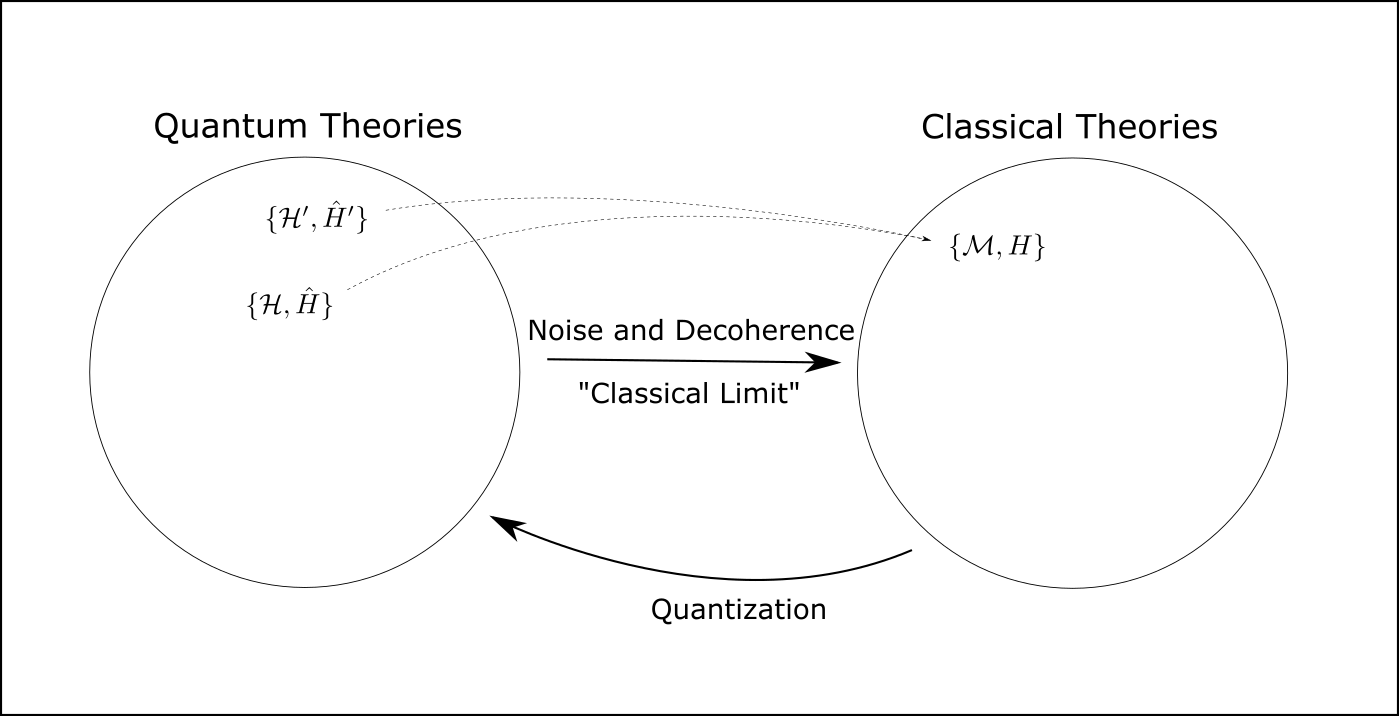
\includegraphics[width=\linewidth]{Figures/fig1.png}
    \caption*{}
    \label{fig:fig11}
\end{figure}
\pagebreak

\subsection{Classical Theory of Identical Particles I}
Why do we want to develop a (classical) theory of identical particles? The answer comes in the form of the Gibbs Paradox. The Gibbs Paradox says that if you have an ideal gas in equilibrium in a container, and you place a barrier into the container, the entropy decreases. This would be bad, because you'd be well on your way to breaking the 2nd law of thermodynamics, and infinite wealth, fame, and glory awaits you. (Un)fortunately, this paradox is resolved if the particles are \textit{indistinguishable}. So first of all, why bother studying these systems of identical particles in any more depth? The answer is that they give us an intuition about what to expect our classical limit to look like. Secondarily, there are many interesting structures that come out of these systems.

Let's begin with a system of $N$ identical classical particles. One's intuition might guess that the phase space of this system is simply the direct product of the individual phase spaces. Let $X$ be the configuration space of this system, and $X_i$ is the configuration space of some $i$'th particle. Then our intuition would tell us that $X = X_1 \times ... \times X_N$. Let $\pi \in S_N$ (where $S_N$ is the symmetry group on $N$ symbols). Then there is no way to distinguish each state $x = (x_1,...,x_N) \in X$ from $x' = (x_{\pi(1)},...,x_{\pi(N)})$ since the particles are identical!  To clarify, we have the following:
\begin{align*}
    x &= (x_1,...,x_N) \\
      &= (x_{\pi(1)}, ... , x_{\pi(N)})
\end{align*}
Let $x, y \in X$. Then we will define an equivalence relation on $X$ given by $x \sim y$ if $(x_1,...,x_N) = (y_{\pi(1)},...,y_{\pi(N)})$. The true configuration space of $N$ particles moving in some system $X$ should therefore be given by the following quotient:
\[\mathcal{M} \equiv X^N / \sim\]
Recall that the elements of a quotient space are the equivalence classes, that is: each element is given by $[x] \equiv \{y | y \sim x\} \in \mathcal{M}$. Typically we abuse notation and write $x = [x]$. If you know about topological spaces, you should by now be saying "uh oh", because quotients do strange things to topological spaces. One of the things a quotient does to a nice topological space is introduce a singularity in the space. We will see this soon. Let's take a simple example: if $X = \RR^n$, then as $S_N$ is a finite group, $\mathcal{M}$ is locally diffeomorphic to $(\RR^n) \times ... \times (\RR^n)$ ($N$ times). What this means is that if you have $N$ particles far away from each other, then it's as if you can look at each particle on it's own. The interesting things happen when particles are near each other, and that's when you get so-called 'singularities'. So let's look at the simplest example we can come up with. $X = \RR$, and $N = 2$.
\pagebreak
\begin{figure}[ht]
    \centering
    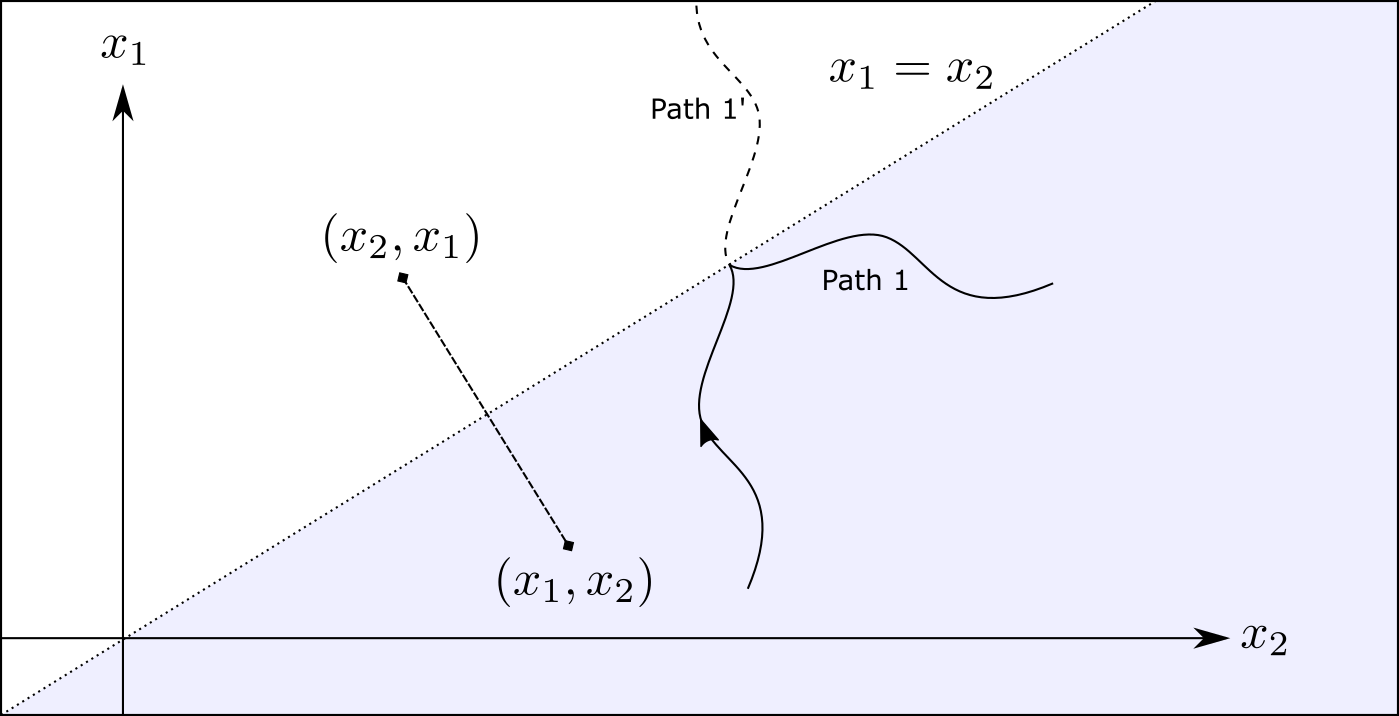
\includegraphics[width=\linewidth]{Figures/figure2.png}
    \caption*{}
    \label{fig:fig12}
\end{figure}

We are going to choose for our representatives of $\mathcal{M} = \RR^2/\sim$ to be the ones given by $x_1 < x_2$. Then an embedding of $\mathcal{M}$ in $\RR^2$ is given by the region $\{(x,y):x<y\}$.

Above is a diagram of our space $\mathcal{M}$ (in blue, embedded in $\RR^2$). We see that in this space, $(x_1,x_2)$ is identified with $(x_2,x_1)$ as $1\mapsto 2$, $2\mapsto 1$ is the only permutation on $\RR^2$. You can see that any point in the interior of the space (completely surrounded in blue) is going to be the same as if it were just in $\RR^2$ - this is what we mean by locally diffeomorphic.


Any path in $\RR^2$ which attempts to cross the line $x_1=x_2$ is going to have something strange happen to it - the path actually reflects, and rather than Path 1' we get Path 1. If you look closely, a tangent vector to the curve undergoes a (discontinuous) reflection when it touches the boundary. This is some interesting behaviour, and demonstrates that our spaces are going to have non-trivial features.
Generally, if $X = \RR^n$ we are going to introduce the center of mass coordinates. If we are in units where each particle has mass $m=1$, then we choose the following:
\[x_{cm} = \frac{1}{N}\sum_{i=1}^N x_i\]
This gives us the result that $\pi(x_{cm}) = x_{cm}$ for any $\pi \in S_N$. What this allows us to do is set $\mathcal{M} = \RR^n \times r(N,n)$, where $r(N,n)$, the \textit{relative space}, encodes the strange global effects we observe of our space, and $\RR^n$ encodes the local information about the space. It turns out that $r(N,n)$ is some $n(N-1)$ dimensional space, but it is not necessarily a differentiable manifold (this is an example of something called an \textit{orbifold}). Now that we have seen the case of $n=1, N=2$, we can move on to arbitrary $n$. Let's analyze the structure of this relative space $r(2,n)$. Let $x_1$ and $x_2$ be the configurations of two particles in $\mathcal{M}$. For our equivalence relation, if we identify $x = x_1 - x_2$ with $-x = x_2 - x_1$, we see that there is one singular point at $0$. In fact, since the equivalence relation simply provides the distance between the two particles in this space as a nice representative, we will see in a second that $r(2,n) \setminus \{0\} = \RR^{+} \times {\RP}^{n-1}$. In general, the section given by $\RR^+$ provides the 'length' of the relative coordinate $x$ (which is why it's called a relative space - this is the distance between the particles), and the other part is something called the real projective space. The simplest examples are $\RP^0$, which is a point, and $\RP^1$, which is a circle. But when $n\geq 3$, $\RP^n$ is a \textit{doubly connected} space, meaning that any closed curve with winding number 2 around the singularity is contractible. The fact that this space is doubly connected (in three dimensions) is important! It will later provide two options for the configuration of a particle, which in turn provides us with two types of particles which we call fermions and bosons. On the other hand, in two dimensions the consequence of $\RP^1$ being a circle is that since the circle is not simply connected, there are interesting phenomena that happen when particles are constrained to move in two dimensions.

Here's a more specific example. Consider two particles moving in $\RR^2$. Then we have $\mathcal{M} = (\RR^2)^{\times 2}/\sim = \RR^2 \times r(2,2)$. It is an exercise to show that $r(2,2)$ is the same as the plane $\RR^2$ with the origin removed and where $x$ is identified with $-x$ (that is, $r(2,2) = \RR^2 / a$, where $a$ is the antipodal map). Below is a rather unsatisfying drawing of this space. You can imagine the bottom of the cone as being the origin. The way that the cone wraps around itself indicates how at each point on the cone, two points of $\RR^2$ are represented - the inside being the negative values and the outside being the positive values.
\begin{figure}[ht]
    \centering
    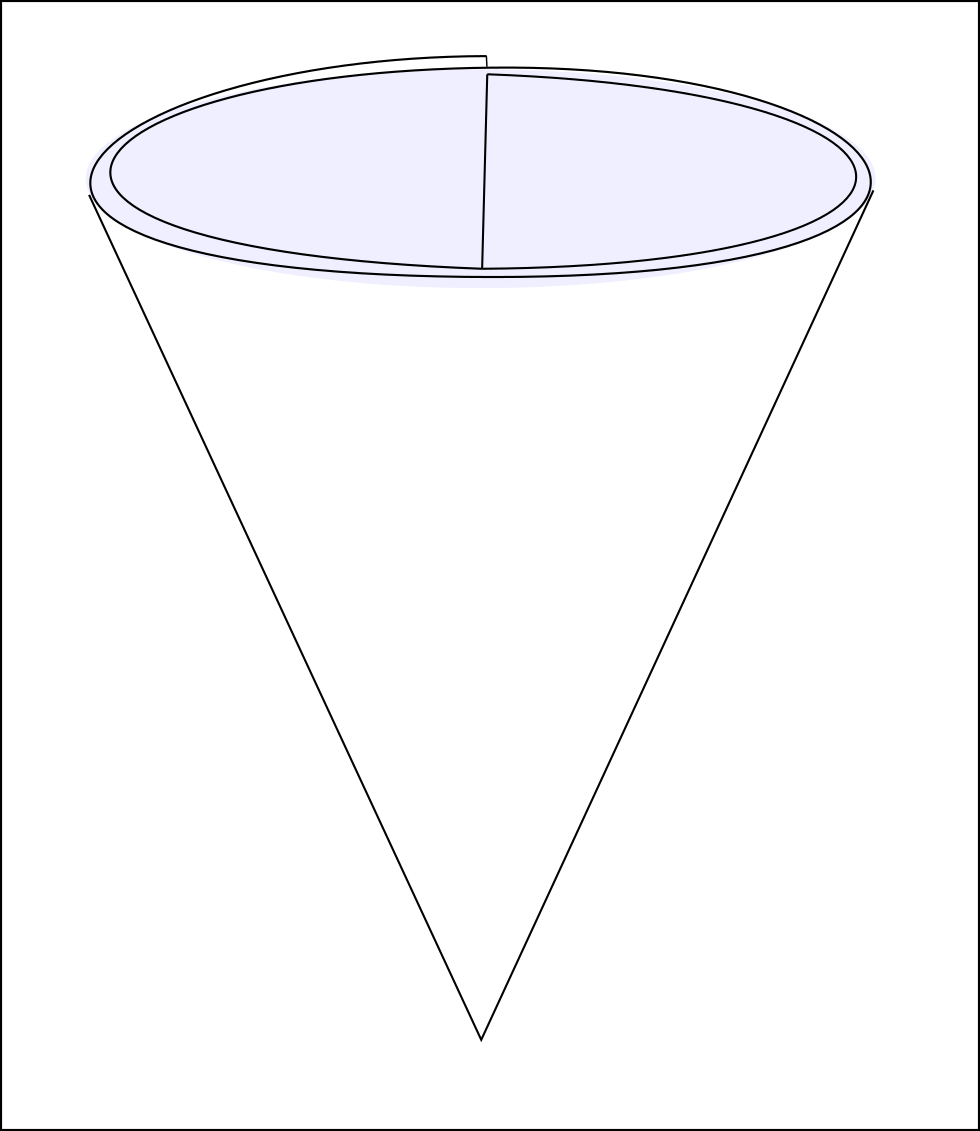
\includegraphics[width=0.5\linewidth]{Figures/rp1.png}
    \caption*{}
    \label{fig:my_label}
\end{figure}
\pagebreak
\section{Relative Space and Quantization}
\subsection{Classical Theory of Identical Particles II}
We noticed in the last section that given a configuration space $\mathcal{M} \equiv (\RR^n)^{\times N}/\sim$, we could rewrite the space in the center-of-mass coordinates to find that $\mathcal{M} = \RR^n \times r(N,n)$, where $r(N,n)$ looks locally like $\RR^{n(N-1)}$ but with a few nasty extra features. The difference between the two manifests in the global (topological/geometric) properties of the spaces. Particularly in the analysis of \textit{parallel transport} and \textit{tangent vectors}. Though we haven't talked in detail about what a tangent vector is, for now we can use our intuition about velocity vectors - it is a vector valued object defined at each point along some curve or surface, and in this particular case we require the vector to be in some sense 'tangent' to the surface. You will see these notions defined in more detail in courses on general relativity or differential geometry, and the geometry of configuration spaces is very closely related to what we call 'gauge theories', which you will see later on as well. If you would like the full picture, it would be beneficial to spend some time studying what is called the \textit{tangent bundle} of a manifold.

\subsubsection{Tangent Vectors}

Let's now use our intuition about velocity to consider some configuration spaces. We say that a velocity vector $v$ is a 'tangent vector to the configuration space', meaning that there is some curve through $\mathcal{M}$ which has velocity $v$ at some point $x$. As an example, in $\RR^2$ a particle requires both position and velocity in order for you to fully specify its' state - we therefore say that the \textit{state} of the particle is the pair $(x,v)$. In a simple space such as $\RR^2$, comparing the velocities of particles is simple, but we often take for granted the process of adding vectors 'tip to tail'. This way of comparing velocities is where you take the velocities as vectors in $\RR^2$ and subtract them pointwise. This works in $\RR^n$ easily, but you have to be more careful when considering so-called 'tangent vectors', which exist in a more complicated space called the tangent space. The tangent space is defined separately at each point in the 'ambient space' (here being \textrm{M}). For $\RR^2$, this is simply $\RR^2$ everywhere. But for an arbitrary manifold $\mathcal{M}$, the tangent space may be different at each point. Therefore we would like a way to transport velocities between tangent spaces in a continuous/parallel way. This is called parallel transport.

\begin{figure}[ht]
    \centering
    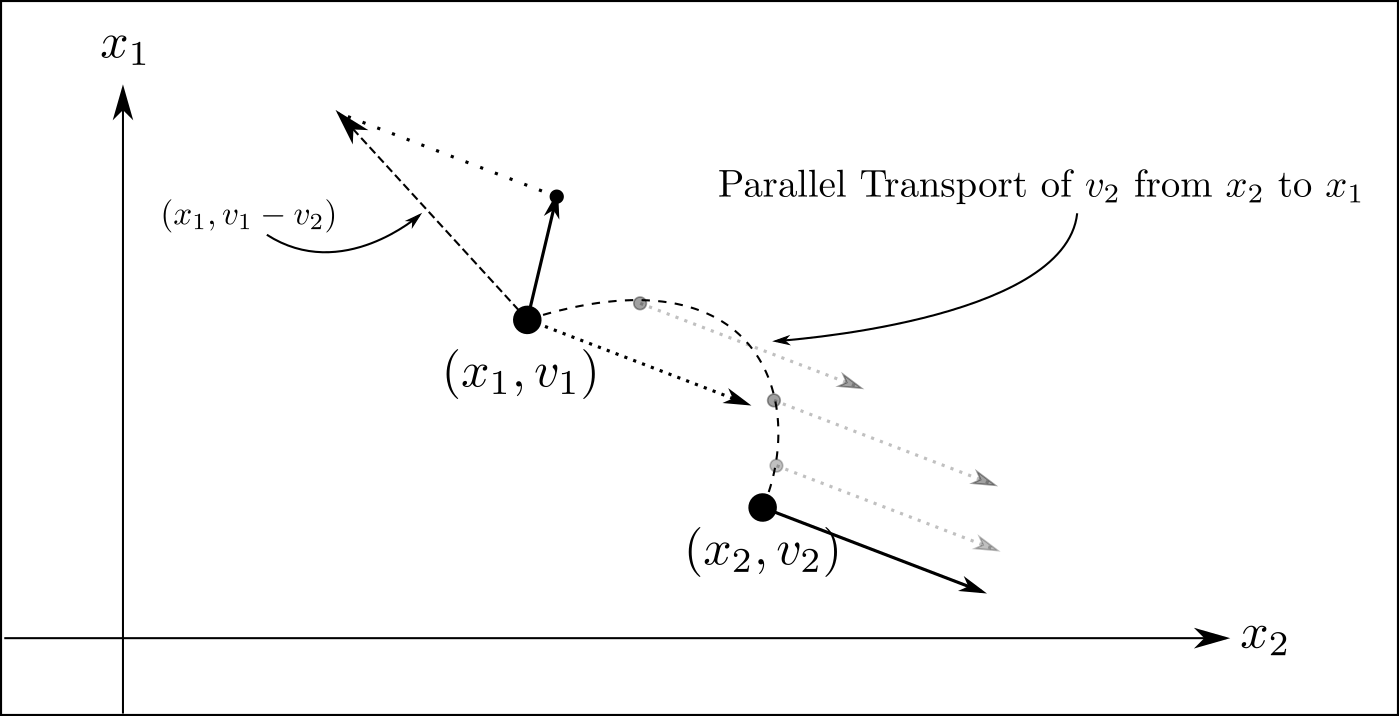
\includegraphics[width=\linewidth]{Figures/figure3.png}
    \caption*{}
    \label{fig:21}
\end{figure}
The above diagram demonstrates this notion of parallel transport in $\RR^2$. Luckily, in euclidean space it does not matter what path we transport $v_2$ along. But there is a simple example where parallel transport fails! Imagine a curve which goes from some point to the north pole, changes direction, comes back down to the original latitude, and goes back to its' origin. A diagram will help.
\begin{figure}[h]
    \centering
    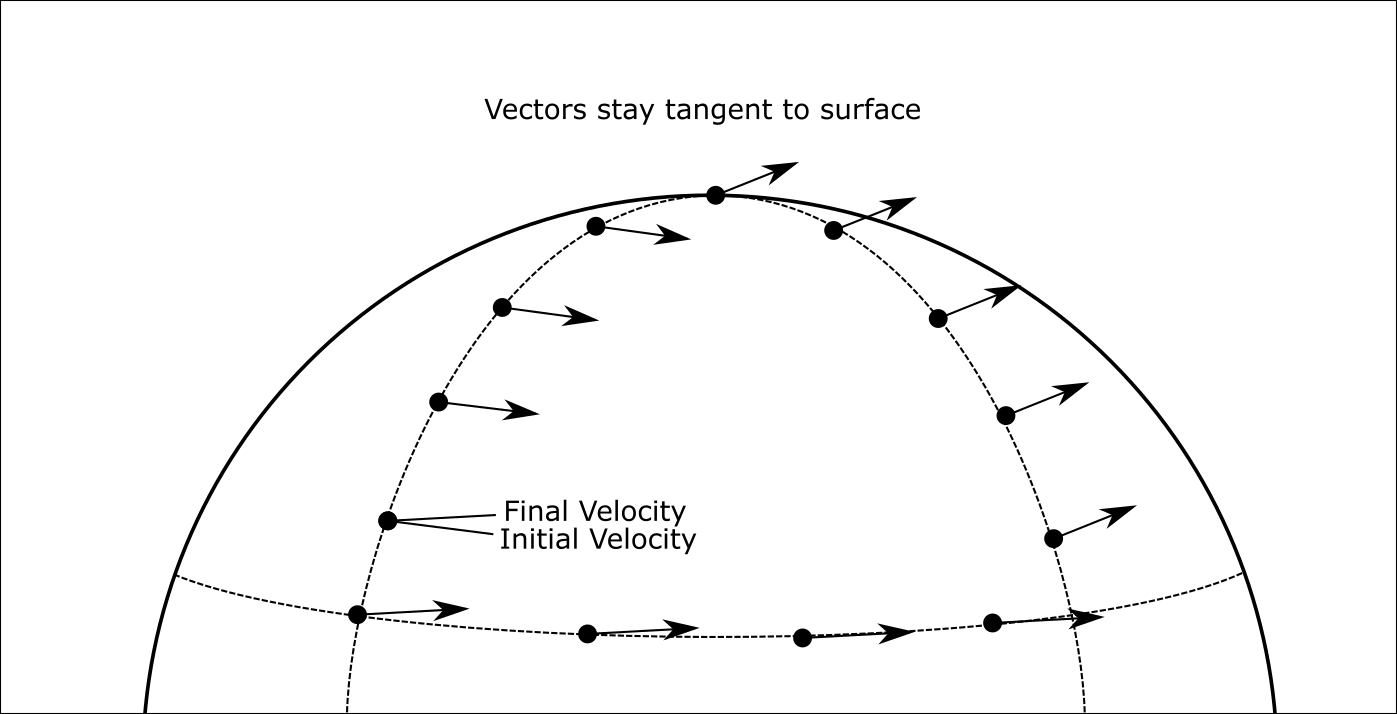
\includegraphics[width=\linewidth]{Figures/spheretransport.png}
    \caption*{}
    \label{fig:22}
\end{figure}

You will notice that if you draw vectors which \textit{stay tangent to the surface of the sphere}, then they change direction slightly as you move across the surface of the sphere. A vector (as shown in the diagram) which starts tangent to a line of latitude will eventually end up being perturbed by the motion.

\subsubsection{Parallel Transport in Relative Space}
Let's consider this parallel transport in our relative space $r(2,2)$, which we saw earlier could be represented as that sort of 'cone' shape. You can check that on an ordinary trajectory on the surface of this cone, vectors do not undergo any strange transformation. But consider when a vector is transported around the singularity. Suppose the trajectory begins at a point $x$, and crosses through the point $-x \sim x$. A vector held parallel along this trajectory is going to have to undergo the transformation $v \mapsto -v$ in order to satisfy the criteria for 'parallel transport'. You can see the reasoning behind this in more detail in any text on Differential Geometry.

Now let's look at three dimensions. We consider the relative space $r(2,3) \cong \RP^2$ of two particles living in three spacial dimensions. A good way to visualize this space (Figure \ref{fig:23} may help in this task) is as follows: imagine the sphere, where each point $x$ is identified with the point on the opposite side of the sphere. As you move towards the equator, you need to identify points on opposite sides of the equator. In this way, it's sort of like the upper half of the sphere (of radius $d/2$, where $d$ is the distance between the particles). There are some great visualizations of this on wikipedia, if you look up 'real projective space'.

The next thing to do would be to try to look at trajectories in this space, so let's consider a few different trajectories, as shown in the next figure.

\begin{figure}[h]
    \centering
    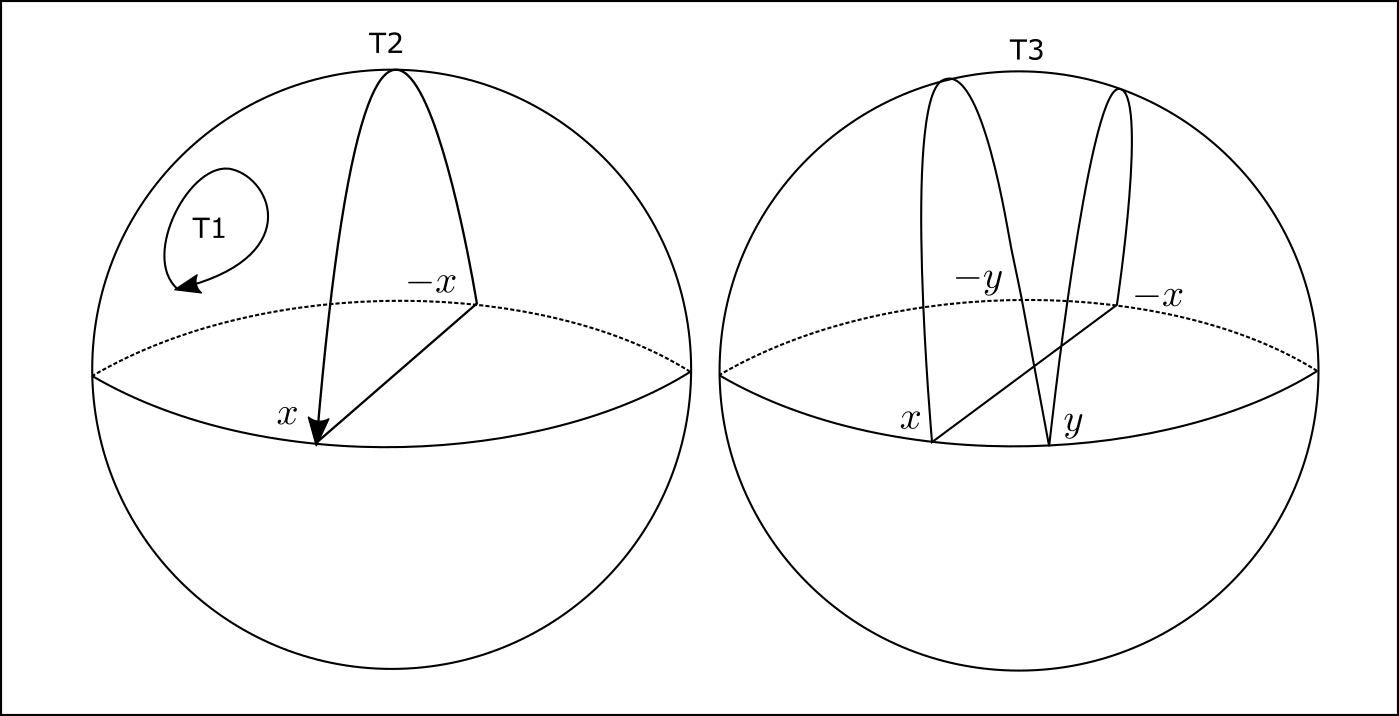
\includegraphics[width=\linewidth]{Figures/trajectories_in_rp2.png}
    \captionsetup{belowskip=-15pt}
    \caption{Graphical representation of $ \mathbb{RP}^2 $}
    \label{fig:23}
\end{figure}

The trajectory T1 is contractible to a point, as this region is clearly simply connected. The trajectory T2 begins at a point on the equator, moves over the surface of the sphere, and then returns to the 'same' point on the other side of the sphere, and the trajectory T3 follows a similar path. It turns out that T3 is contractible to a point, but T2 is not! The reason for this is that T3 passes around the singularity twice, whereas T2 only passes around the singularity once. A space like this is called \textit{doubly connected}, and can be studied in detail in a Topology course. 

Now, why did we spend so much time going over these weird properties? I hope this sets the stage for the study of the mysterious properties of these configuration spaces, but these properties don't have much of an effect in classical mechanics. This is because classical mechanics is very local. The place where this becomes much more important is in quantum systems. So we are now going to leave the topic of classical particles, and begin the study of quantum point particles.

\subsection{Quantization of Identical Quantum Particles I}

We need to remember that the problem of quantization is not very well posed. Many quantum systems can result in the same classical system, so we need to consider some guiding principles. As as example, if our configuration space $\mathcal{M}$ is continuous, we should take $L^2(\mathcal{M})$ as our Hilbert space - this is a very common approach. But we know that this is just one example of a probabilistic theory - there are quite a few structure that could give the same probabilistic data for a system, so we need to answer a specific question: \textbf{What do we mean by wavefunction?} A very literal approach would be that a wavefunction is a function! 
\[\Psi: \mathcal{M} \to \CC\]

But there is an alternative interpretation to the word wavefunction, and it can give inequivalent results! Let's construct it. First we need to build some space $E$ which is locally similar to $\mathcal{M} \times \CC$ (it could just be $E \cong \mathcal{M}\times \CC$). As an example, we could take $\mathcal{M} = \RR$. A trajectory in $E \cong \RR \times \CC$ would be equivalent to what you've learned in single particle 1D quantum mechanics - below is a diagram of what this looks like. But this construction becomes different when you start looking at spaces which have singularities and other strange properties. So let's put some terminology together.

The space $\mathcal{M}$ is called the \textit{base space}. The space $\CC$ is called the \textit{fibre}. The space $F$ is called the \textit{fibre bundle}, and a choice of an element in $\CC$ for each point in $\mathcal{M}$ is called a \textit{section}. Since our fibre is $\CC$, we will just call this a $\CC$-bundle.

\begin{defn}[Vector Bundle]
Let $\mathcal{M}$ be a manifold. Suppose for each point $x \in \mathcal{M}$ we associate a vector space $h_x$. We define a vector bundle over $\mathcal{M}$ to be the disjoint union $\sqcup_x h_x = E$. This definition provides the existence of a projection $\pi : E \to \mathcal{M}$ given by $\pi(x,h_x)=x$.
\end{defn}


\begin{defn}[Section]
	Suppose $E$ is a vector bundle over $\mathcal{M}$. A section of $E$ is a map $\Psi : \mathcal{M} \mapsto h_x \in E$, so that $\Psi(x) = \psi(x)\chi_x$. The set of all sections of $E$ is denoted $\Gamma(E)$.\footnote{In the case $E=T\mathcal{M}$ (the tangent bundle), we write $\Gamma(TM) = \mathfrak{X}(M)$}
\end{defn}

\begin{defn}[$\CC$-Bundle]
	A $\CC$-bundle over a manifold $\mathcal{M}$ is a vector bundle $E$ where each $h_x \in E$ has $h_x \cong \CC$.
\end{defn}

So that's one interpretation of a wavefunction - it's a section of a $\CC$-bundle over a base space $\mathcal{M}$ (provided the section meets some continuity and differentiability requirements, which won't be discussed in depth). Why go through these complicated constructions with all this terminology? Because there are sometimes multiple nontrivial $\CC$-bundles over a space which are \textit{inequivalent}! We can even go further, as a nice example we can consider relatively simple spaces over which there are inequivalent $\RR$-bundles (fibre bundles where the fibre is $\RR$). We could consider "real" quantum mechanics, where every wave function is real-valued. There are some problems with the theory of real quantum mechanics (mostly with entanglement), but it's a perfectly respectible theory in many ways. So consider the base space $\mathcal{M} = S^1$, the circle. We will construct two different $\RR$-bundles over the circle, which are shown on the following page in a diagram from the Encyclopedia Britannica.

\begin{figure}[h]
    \centering
    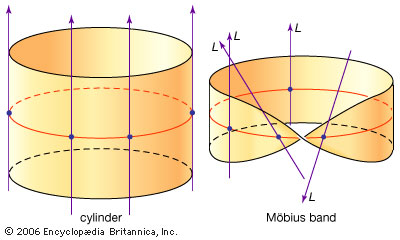
\includegraphics[width=\linewidth]{Figures/mobius_bundle.jpg}
    \caption*{}
    \label{fig:24}
\end{figure}

In order to describe wavefunctions as sections of these bundles, it's therefore important to consider the vector space properties of $\CC$, as you could choose some basis vector for the fibre and it will twist and turn as you move around the base space. The way we do this is to further generalize our fibre bundle. Let's just consider our base space $\mathcal{M}$, and for each point $x$ in $\mathcal{M}$ we will associate a fibre $h_x$. In our case, we will always be using $\CC = h_x$, but it's important to make this generalization so that we can write the following. We want to make some choice of (normalized) basis vector $\chi_x$ for each $h_x$, so that $\textrm{Span}(\chi_x) = h_x$. Thus any section $\Psi$ can be written so that you can evaluate $\Psi$ at a point: $\Psi(x) = \psi(x)\chi_x$. You could therefore change this basis vector as you move around the space! Such a choice of $\chi_x$ for each $h_x$ is called a choice of gauge, and it's the same gauge you refer to in gauge theory. Suppose you wanted to change your basis vectors, so that 
\[\left\{\chi_x \right\} \mapsto \left\{\chi_x'=e^{-i\varphi(x)}\chi_x\right\}.\] 
Then you'd require that $\psi'(x) \mapsto e^{i\varphi(x)}$ so that $\Psi$ is unchanged. This is called a gauge transformation. The fact that physical quantities should not depend on this choice of gauge (gauge invariance!) causes issues when defining your derivative operator, and we will talk about this in the next section.

\subsection{Quantization of Identical Quantum Particles II}
We won't spend too long talking about the theory of $\CC$ bundles. In this lecture we will move towards understanding identical particles, types of identical particles, and how to describe them in quantum mechanics. Today is the last day we will talk about understanding how there can be more than one quantization for a given classical system, due to this description in terms of $\CC$ bundles. So let's get into it. Here's some recap of the previous section.

Recall that a \textbf{State} is an assignment of complex vectors at each point in $\mathcal{M}$, or in other words, it is a section of a $\CC$-bundle over $\mathcal{M}$. To do computations with this on a computer, we need to choose a basis for each point in the $\CC$-bundle. Such a choice of basis is called a \textit{frame}.

\begin{defn}[Frame]
	Given a fibre bundle $E$, A \textit{local frame} for $E$ on some open set $M \subseteq \mathcal{M}$ is a choice of basis $\chi_x$ for each $h_x \in E$, with $x \in M$.
\end{defn}

\begin{defn}[Quantum State]
	A state $\Psi(x)$ of a quantum system is a \textit{section} of a $\CC$-bundle over the configuration space $\mathcal{M}$ of the system.
\end{defn}

Let $h_x$ be the fibre at the point $x \in \mathcal{M}$. Then we can choose a normalized basis vector for $h_x$ denoted $\chi_x$. Recall that for $\RR$ we can only choose $1$ or $-1$ to be our normalized basis vectors, but in $\CC$ we can choose $e^{i\phi}$ to be our normalized basis vector.

Once we've chosen this basis $\chi_x$ then we could write $\Psi(x) = \psi(x) \chi_x$.

We want to understand how to keep our quantities invariant to our choice of basis. So let's recall the \textit{Gauge Transformations}, which are transformations of the form $\chi'_x = e^{-i\phi(x)}\chi_x$. Under a gauge transformation, $\Psi$ is transformed by $\Psi'(x) = \Psi(x) \exp(i\phi(x))$. The clear example of a gauge invariant quantity is the probability amplitude $p(x)$; we have, in fact, 
\[p'(x)= \overline{\Psi'(x)}\Psi'(x)= \overline{\Psi(x)} e^{-i\phi(x)}e^{i\phi(x)}\Psi(x)=\overline{\Psi(x)}\Psi(x)=p(x)  \]

 This is expected. But we'd also like to look at other quantities, such as our position and momentum operator.

\begin{defn}[Gauge Transformation]
	A gauge transformation $U$ is a choice of maps $U_x : h_x \to h_x$ with $U_x(\chi_x) = e^{-i\phi(x)}\chi_x$. This induces a transformation on sections of $E$ as so: $U[\Psi](x) = e^{i\phi(x)}\Psi(x) $
\end{defn}

\subsection{Making Momentum Gauge Invariant}

Let's try to show that the momentum operator (that we learned about originally) is not gauge invariant. Recall that (in natural units) $\hat p = -i \pdv{x^k}$

\[\hat p \Psi' = -i \lim_{\epsilon \to 0}\frac{e^{i\phi(x+e_k\epsilon)}\Psi(x+e_k\epsilon) - e^{i\phi(x)}\Psi(x)}{\epsilon}\]

We remark that $\phi(x+e_k \epsilon)$ and $ \phi(x)$ are completely uncorrelated and in the limit of $\epsilon \to 0$ it is not guaranteed that they are equal! 
We didn't require $\phi$ to be continuous. What this means is that we could set up an experiment to measure $\phi$ and recieve information about gauge, which means that this formulation is not independent of our choice of basis. The next step is to therefore develop a new notion of momentum.

\subsubsection{Using Parallel Transport}

As we saw in the previous section, parallel transport provides a nice way of comparing two tangent vectors (in this case the gauge $\chi_x$) in order to develop a new difference quotient. Let's look more closely at the precise definition of parallel transport. 

Recall that to parallel transport a vector in a tangent space $h_x$ into a different space $h_y$. Therefore we'd like a map (preferably a linear one!) that transports these vectors. This map will of course depend on the path $\gamma(t)$ between $x$ and $y$, and we will denote it $P_\gamma(y,x)$\footnote{This map will also often be denoted $\Gamma(\gamma)_x^y$, for example on wikipedia.}.

\begin{defn}[Parallel Transport Map] The parallel transport map is a linear map $P_\gamma(x,y) : h_x \to h_y$, with the following additional properties.
\begin{itemize}\setlength\itemsep{0.5em}
\item$ P_\gamma(x,x) = \mathbb{I}$
\item$ P_\gamma(y,z) \circ P_\gamma(z,x) = P_\gamma(y,x)$
\item$ P_\gamma(y,x)$ is an isomorphism (with $P_\gamma(x,y)=P^{-1}_\gamma(y,x)$)
\end{itemize}
\end{defn}
 
We would like $P_\gamma(y,x)$ to be gauge invariant so that the following holds:

\begin{equation}
P_\gamma(y,x) \mapsto e^{-i\phi(y)}P_\gamma(y,x) e^{i\phi(x)}
\end{equation}

We would also like to see that $P_\gamma(y,x) \to \mathbb{I}$ as $y \to x$ as long as $\gamma$ is a sufficiently well behaved path (that is, it's the most "direct path" between the two points) \footnote{a minimal geodesic}. In other words, $P_\gamma(x+dx,x) \approx \mathbb{I} - i \dd x^k b_k(x)$, where $b_k$ are the relevant taylor expansion coefficients. 

This discussion of parallel transport leads us to our next definition, the covariant derivative. This is a method of differentiating vector fields (ie, sections of vector bundles) which leaves the structure of a manifold intact.

\begin{defn}[Covariant Derivative]
Let $\mathcal{M}$ be a manifold with $\CC$-bundle $E$. Suppose there is a suitably well behaved parallel transporter $P$ on $E$, and that $\Psi \in \Gamma(E)$. The covariant derivative in the direction of $e^k$ is denoted $D_k$ and is defined as follows.
\begin{align}
D_k \Psi(x) &= \lim_{h \to 0} \frac{P_\gamma (x,x+h e^k) \Psi(x+he^k) - \Psi(x)}{h}\\
	&= \lim_{h \to 0}\frac{(\mathbb{I} - i h e^k b_k(x))\Psi(x+ he^k) - \Psi(x)}{h}\\
	&= \left[\pdv{x^k}-ib_k(x)\right]\Psi(x)
\end{align} 
\end{defn}

\begin{exercise}
	Determine how $b_k(x)$ transforms under a gauge transformation $ \chi_x' = e^{-i\phi(x)}\chi_x $ 
\end{exercise}
\begin{exercise}
	Show that $D_k$ is gauge invariant.
\end{exercise}

\begin{exercise}
	Show that for a single particle with spin, the Hamiltonian $\sum_k \frac{-1}{2m} D_k^2 = H$ is equivalent to that given by a static magnetic field (this tells us how such geometric changes could be induced experimentally). In the end, you will learn that these $b_k(x)$ are similar to the choice of magnetic field - they are related to the gauge field $A$.
\end{exercise}

The issue with this is that we want particles to locally behave like free particles - we don't want particles on their own in the middle of nowhere to act as if they are in magnetic fields. So we need to choose $b_k(x)$ so that the 'ficticious' magnetic force is zero. For nontrivial geometries, there do exist choices of $b_k(x)$ so that the force field will vanish (that is - the curvature tensor associated with the ficticious field vanishes). You may recall this expression from electrodynamics (it essentially says that $A$ is curl-free, or that $B=0$).

\begin{equation}
f_{k\ell}(x) = i[D_k,D_\ell] = \pdv{b_\ell}{x^k} - \pdv{b_k}{x^\ell}=0
\end{equation}

As long as equation 5 is imposed everywhere (except singularities, such as is the case on $\mathcal{M}=r(2,2)$) we will have freedom in choosing the $b_k$ terms. This freedom at the singularities allows us to pick nontrivial $b_k$ terms, which gives rise to interesting phenomena in 2-d materials. Due to $b_k$ being curl free, we also now know that $P_\gamma(y,x)$ is path independent as long as $\gamma$ does not encircle the singularity.

Let's study what happens when you go in a loop around the singularity. You can see that $P_\gamma(x,x)$ should just be some number $e^{i\xi}$ for some $\xi \in [0,2\pi)$, as $h_x \cong \CC$ and $\dim(\CC)=1$. However, this $\xi$ turns out to be independent of $x$! Consider now Figure \ref{fig:31}. 

\begin{figure}[ht]
    \centering
    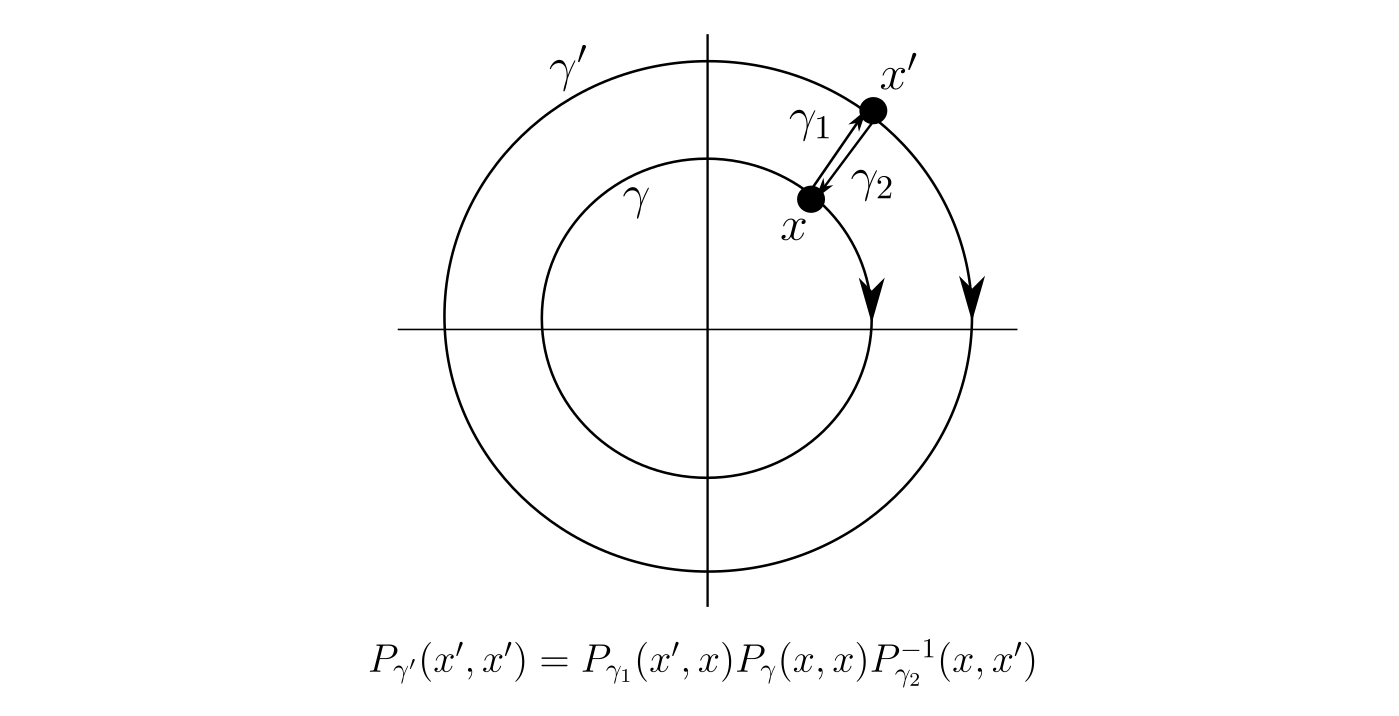
\includegraphics[width=\linewidth]{Figures/path_independence_gauge.png}
    \captionsetup{belowskip=-15pt}
    \caption{The two paths $ \gamma $ and $ \gamma' $ belong to the same homotopy class and then the above identity must hold.}
    \label{fig:31}
\end{figure}

So when $e^{i\xi}=1$, nothing happens when you move around a singularity - this means the wavefunction is unchanged! However, when $e^{i\xi}\neq 1$, you will be able to generate phases of $e^{i\xi n}$ for any $n \in \ZZ$ by transporting vectors around the singularity. This means that if you have some strange system with $e^{i\xi}\neq 1$ then dynamical effects will be observable due to the geometry of the system. This can only happen in two spacial dimensions!

\subsection{Free Particle in Two Dimensions}

Now let's consider the free particle in two dimensions. We will neglect center of mass coordinates, and use polar coordinates. The standard hamiltonian for a free particle in two dimensions is the following.

\begin{equation}
H = \frac{-1}{m}\left(\pdv[2]{r}+\frac{1}{r}\pdv{r}+ \frac{1}{r^2}\pdv[2]{\phi}\right)
\end{equation}

When you have this property that wavefunctions pick up a phase of $e^{i\xi}$ when you go around the singularity, you impose a nontrivial boundary condition: $\Psi(r,\phi+2\pi) = e^{i\xi}\Psi(r,\phi)$. This is what gives us strange dynamics - polar coordinates no longer gives us nice symmetry. 

\paragraph*{Alternative approach}

There is, however, a transformation you can make to the Schrodinger equation that makes it easier to solve. The strategy is to replace $\Psi$ with $\Psi'(r,\phi) = e^{i\frac{\xi}{2\pi}\phi}\Psi(r,\phi)$. Then the Hamiltonian transforms as $H' = e^{-i\frac{\xi}{2\pi}\phi}H e^{i\frac{\xi}{2\pi}\phi}$. This gives $H\Psi = H'\Psi'$, so the solutions to the Schrodinger equation are unchanged. But observe what happens:

\begin{equation}
H' = \frac{-1}{m}\left(\pdv[2]{r}+\frac{1}{r}\pdv{r}+ \frac{1}{r^2}\left(\pdv{\phi}+\frac{i\xi}{2\pi}\right)^2\right)
\label{eq:Hamiltonian_gauge_invariant}
\end{equation}

\begin{exercise}
	Solve the Schr\"odinger equation for $ H $ (via $ H' $ in Eq. \eqref{eq:Hamiltonian_gauge_invariant}).
\end{exercise}

\subsection{Particle Statistics}

This weirdness doesn't happen in three dimensions. The reason is that $\RP^{n-1}$ is doubly connected. Any curve $\gamma^2$ that goes around the singularity twice is contractible. Therefore we have $P_{\gamma^2}(x,x) = e^{2i\xi}=1$, so $\xi = 0$ or $\xi = \pi$. In the case that $\xi = \pi$, we have the dynamics of a fermion. In the case that $\xi = 0$ we have the dynamics of a boson! But what does it mean to go around the singularity once in $\RP^{n-1}$? It means you exchange the two particles. This is why fermions are antisymmetric under exchange, which is what causes the Pauli exclusion principle. We will see this in extreme detail in the following lectures.

\section{Fock Space}
In the previous three lectures we've been looking at the quantum theory of identical particles in 3D. You can see what we've covered in these lectures as the tip of a very large iceberg, which as a society we've only really begun to explore. What we have a good understanding of is the theory of identical point particles in 3 spacial dimensions or higher. What we have begun to uncover is the theory of extended, or membrane-like, interacting particles (ie, strings and so on). This falls under the title of "modular tensor categories". We will move on from this, but I wanted to make you aware before we move on that this field is still being studied extensively even now.

Another subject, very closely related - being the tip of this iceberg, is the study of Fock space and 'second quantization'. This is what we will cover for the next few lectures.

\subsection{Symmetric and Antisymmetric Representation}

We've learned about single particles in our elementary quantum mechanics course. What we would like to do is work out the Hilbert space to assign to a system of multiple particles provided that each of the particles has some Hilbert space of states $H$. Well, what we do know is the Hilbert space for N distinguishable particles, let's call it $\Hh$.
\begin{equation}
\Hh = H^{\otimes N} =: \bigotimes_{i=1}^N H
\end{equation}
But this space is too big to be what we want for indistinguishable particles. There are states in this space which would be physically the same. As an example, if you consider these to be position states of particles, then exchanging two particles would produce a positive or negative sign - in the case of a Boson there would be degeneracy here as the states would be identical.

We will use this information we learned - that $\ket{x_1,x_2} = \pm \ket{x_2, x_1}$ - and turn it into a way to reduce our Hilbert space to be something smaller. Of course, there is more information we could consider - such as when a particle has internal degrees of freedom such as spin. These are called parastatistics, but we won't cover them in this course.

The best way to reduce our model is to find a subspace of $\Hh$ which corresponds to exactly the unique configurations. There is a direct connection here between quantum theory and the representation theory of $S_N$ on $N$ symbols. This motivates us to define a representation.

\begin{defn}
Suppose $G$ is a group.\footnote{A group $G$ is a set endowed with an operation which takes two elements of $G$ and produces a third. This operation must be invertible (in the sense that there exists $a^{-1}$ for every $a$, and there must be an identity. We also require this operation to be associative.} A representation $U$ of $G$ over some vector space $V$ is a group homomorphism $U:G \to B(V)$, where $B(V)$ is the group of bounded linear operators on $V$.
\end{defn}

There are multiple definitions of a representation, but it doesn't matter here. We will focus on unitary representations since in this course we will usually consider transformations which correspond to unitary representations of some group. That is to say, we would like $U(g)$ to be unitary for any $g \in G$. There is a natural action of $S_N$ on $H^{\otimes N}$ given as follows.

\begin{equation}
U(\sigma)\ket{x_1,...,x_N} = \ket{x_{\sigma(1)},...,x_{\sigma(N)}}
\end{equation}

This action extends by linearity to our entire space (ie $U(\sigma)(a\ket{\psi}+b\ket{\phi}) = aU(\sigma)\ket{\psi}+bU(\sigma)\ket{\phi}$). What we should do, even though it is a tedious exercise, is write down a matrix for an example and see where that takes us.

Consider the permutation $\pi(1,2,3)=(3,1,2)$. We'd like to see the representation of this matrix on some space. Let's pick $\CC^2$ as our $H$, and $\Hh=H^{\otimes 3}$. Fix a basis $\ket{0},\ket{1}$ for the individual space. Then a basis for $\Hh$ is given as:
\[\ket{000},\ket{001},\ket{010},\ket{011},\ket{100},\ket{101},\ket{111}\]

Then a matrix representation for $\pi$ is given as follows.

\[U(\pi) =  \begin{bmatrix}
1&0&0&0&0&0&0&0\\
0&0&1&0&0&0&0&0\\
0&0&0&0&1&0&0&0\\
0&0&0&0&0&0&1&0\\
0&1&0&0&0&0&0&0\\
0&0&0&1&0&0&0&0\\
0&0&0&0&0&1&0&0\\
0&0&0&0&0&0&0&1
		\end{bmatrix}= \mathbb{I}\oplus
\begin{bmatrix}
0&1&0&0&0&0\\
0&0&0&1&0&0\\
0&0&0&0&0&1\\
1&0&0&0&0&0\\
0&0&1&0&0&0\\
0&0&0&0&1&0
\end{bmatrix}\oplus\mathbb{I}\]

You will notice that this matrix was block diagonal (to an extent). It is usually nice to look for bases where our matrices decompose into direct sums (or bases where our matrices can't be decomposed at all!). Such a choice of basis where matrices can't be decomposed into blocks (ie, a choice of representation associated with that basis) is called an irreducible representation. Let's move on now.

Since our particles are indistinguishable, there is no physically realizable experiment which could distinguish between two identical states. This means that for any observable $A$, we must have $U(\pi) A = A U(\pi)$ for all $\pi$. A very special role is played by vectors $\ket\psi$ such that $U(\pi) \ket{\psi} = \pm \ket{\psi}$. If we rewrite this in a peculiar way: $U(\pi)\ket{\psi} = u(\pi)\ket{\psi}$, you will see that this is an eigenvalue equation. We are searching for subspaces of $H^{\otimes N}$ which are simultaneous eigenspaces of all the permutation operators. The first thing we should argue is that this $u(\pi)$ is itself a representation of $S_N$ on $\CC$. We argue this because you will note that $U(\pi_1\pi_2) = u(\pi_1)u(\pi_2)$. Our claim is that there are only two distinct one-dimensional representations of the symmetric group. The proof is as follows.

Recall that every element of $S_N$ can be written as a product of other elements: $\pi = \tau_{ij} \circ ... \circ \tau_{k\ell}$ where each $\tau_{ij}$ is a 'transposition' (ie, for $\tau_{ij}(\ell)$ takes $i \to j$ and $j \to i$, and $\ell \to \ell$ if $j\neq \ell \neq i$). Thus we can deduce that for any one-dimensional representation of $S_N$ we have $u(\pi) = \prod_k u(\tau_{ij_k})$. This means that all one-dimensional representations are entirely characterized by the representations of the transpositions. We can try something else as well: note that $u(\pi)u(\tau_{ij})u(\pi^{-1}) = u(\pi\circ \tau_{ij}\circ \pi^{-1}) = u(\tau_{\pi(i)\pi(j)}) = u(\tau_{ij})$ (think about it for a minute). But for any $i,j$ there is some permutation so that $\pi(i,j) = (1,2)$! So we have completely characterized all representations by specifying $u(\tau_{12})$. We also know that $u(\tau_{12})^{2} = 1$, as transpositions are their own inverse, so there are only two possible solutions to this equation: $u(\tau_{12})=\pm1$. This completely determines all one-dimensional representations of $S_N$.
\begin{defn}[Trivial Representation]
The trivial 1D representation of $S_N$ is $u$ so that $u(\tau_{12}) = 1$. This means that $u(\pi) = 1$ for all $\pi \in S_N$.
\end{defn}
\begin{defn}[Antisymmetric Representation]
The antisymmetric representation of $S_N$ is $u$ so that $u(\tau_{12}) = -1$. This means that for any $\pi \in S_N$ we have $u(\pi) = \sgn(\pi)$.
\end{defn}

There is a fancy notation we can use in order to cover both cases at the same time - this way we don't need to always worry about which representation to deal with. Let's define $s$ as follows.
\[s(\pi)=\begin{cases}1 & u(\tau_{12})=1\\
\textrm{sgn}(\pi) & u(\tau_{12})=-1
\end{cases}\]
\pagebreak

\subsection{Antisymmetric/Symmetric Space}
Now that we have some machinery developed to study Bosons and Fermions, let's look at the following construction.
\begin{equation}
P_{+} = \frac{1}{N!}\sum_{\sigma \in S_N} U(\sigma)
\end{equation}
\begin{equation}
P_{-} = \frac{1}{N!}\sum_{\sigma \in S_N} \sgn(\sigma) U(\sigma)
\end{equation}
First of all, it's not clear what exactly these matrices are. What we see is that they are big sums of unitary matrices, but are they Hermitian? Unitary? What are they? We claim that these are both projections. That is: $P_{\pm}^2 = P_{\pm}$. We go through the proof of the first case, leaving the second as an exercise.
\[P_+^2 = \frac{1}{(N!)^2} \sum_{\pi,\pi'}U(\pi)U(\pi') = \frac{1}{(N!)^2}\sum_{\pi,\pi'} U(\pi \circ \pi')\]
Let $\sigma = \pi\circ \pi'$. Then we have:
\[P_+^2 = \frac{1}{(N!)^2} \sum_{\sigma,\pi^{-1}}U(\sigma) = \frac{1}{(N!)^2}\sum_{\sigma}U(\sigma) \sum_{\pi^{-1}}1 = \frac{1}{N!}\sum_{\sigma} U(\sigma) = P_+\]

Since these operators are projections, this tells us they have some associated invariant subspace $V$ where $P_\pm (V) = V$. Let's name these subspaces.
\begin{defn}[Symmetric/Antisymmetric Space]
We define the antisymmetric and the symmetric Hilbert spaces in the following formula.
\begin{equation}
\Hh_\pm^N = P_\pm(\Hh) = P_\pm(H^{\otimes N})
\end{equation}
\end{defn}
We see the following properties arise from these subspaces. 

Let $\ket{\psi} \in H_-^N$. Then $U(\tau_{12}) \ket{\psi} = U(\tau_{12}) \frac{1}{N!}\sum_{\pi}\sgn(\pi)U(\pi) \ket{\psi}$
\[U(\tau_{12})\ket{\psi} = \frac{1}{N!}\sum_{\pi'}\sgn(\tau_{12}^{-1}\circ \pi')U(\pi') \ket{\psi} = \frac{1}{N!}\sum_{\pi'}\sgn(\tau_{12})\sgn(\pi')U(\pi')\ket{\psi}=-\ket{\psi}\] Similarly, for any $\psi \in \Hh_+^N$, $U(\pi)\ket{\psi} = \ket{\psi}$. This essentially gives us a way of defining Fermions and Bosons rigorously as elements of subspaces of an abstract Hilbert space.
\pagebreak

Let's introduce some shorthand notation.
\[H_s^N = \begin{cases}H_+^N & \textrm{ for bosons} \\ H_-^N & \textrm{ for fermions}\end{cases}\]
With $s = +1$ when we talk about Bosons and vice versa for Fermions.
\subsection{Definition of Fock Space}
Now we would like to generalize from a space with $N$ particles to a space with arbitrary numbers of particles. This way we can introduce or remove particles from our system. In fact, we can even allow $N$ itself to be a quantum number, and allow superpositions of states with differing numbers of particles! This leads to a process commonly known as Second Quantization whereby the notion of a 'particle' itself changes significantly. The space which allows this is called Fock Space, with the following definition.

\begin{defn}[Fock Space] We define the symmetric/antisymmetric Fock Space $\Gamma_s(\Hh)$ as the direct sum of all the individual Hilbert spaces.
\begin{equation}
\Gamma_s(\Hh) = \bigoplus_{N=0}^\infty \Hh_s^N =: \bigoplus_{N=0}^\infty \Gamma_{s,N}(\Hh)
\end{equation}
\end{defn}
Note that we define $H_s^0$ to be $H_s^0=:\CC$. This is the 'vacuum' space, with basis vector $\ket{\Omega}$, which is the vacuum state. It is the state of the system when there are no particles at all.

Recall that we can decompose a vector into it's components in a space. Let's do this for an arbitrary state $\ket{\psi} \in \Gamma_s(\Hh$. We see that $\ket{\psi} = \sum_{n=0}^\infty\sum_{i=0}^n \psi_n \ket{\phi_i}$, where each $\ket{\phi_i}$ is a basis vector from $\Gamma_{s,N}(\Hh)$. It is easy to see that $\Gamma_{s,N}(\Hh)$ is a separable space, but it remains to be shown that there is an inner product on this space. We will simply write $\ket{\psi} = \sum_{n=0}^\infty \ket{\psi_n}$ for the components of a vector in Fock space instead. Thus the scalar product on this space is $\braket{\psi}{\phi}=\sum_{n=0}^\infty \braket{\psi_n}{\phi_n}$. Now let's look at some observables on this space! What could we measure? The first one that comes to mind is the particle number operator $\hat N$.
\begin{defn}[Number Operator]
We define the particle number operator $\hat N$ as follows.
\begin{equation}
\hat N \ket{\psi_N} = N\ket{\psi_N} \forall \psi_N \in \Gamma_{s,N}(\Hh)
\end{equation}
\end{defn}
This way, states of determinate particle number are states where the only components are members of a subspace comprised of states with exactly $N$ particles. 

\subsection{Dynamics in Fock Space}
Now we would like to see what happens when we change the space according to some dynamics. That is, we want to look at maps $A : \Hh_1 \to \Hh_2$ and extend them to maps between different Fock spaces. This will allow us to define time evolution and so on. Well, we know how to produce from $A$ a linear operator from $\Hh_1^{\otimes N} \to \Hh_2^{\otimes N}$. We just tensor $A$ together $N$ times.
\[A^{\otimes N} : \Hh^{\otimes N}_1 \to \Hh_2^{\otimes N}\]
It turns out that the tensor product of operators respects antisymmetry and symmetry. That is to say, $A^{\otimes N}(\Gamma_{s,N}(\Hh_1)) = \Gamma_{s,N}(\Hh_2)$. You may recall this from previous studies of tensors. This comes from the fact that $[U(\pi),A^{\otimes N}] = 0$. We introduce some notation now.
\begin{equation}
\Gamma_{s}(A) : \Gamma_{s}(\Hh_1) \to \Gamma_s(\Hh_2)
\end{equation}
This definition is given by the following:
\begin{equation}
\Gamma_s(A) = \bigoplus_{N=0}^\infty \Gamma_{s,N}(A) =: \bigoplus_{N=0}^\infty A^{\otimes N}
\end{equation}
Where $\oplus$ here is the matrix direct sum. If you think of $A$ as performing some kind of operation on vectors, say a rotation or something. Then we can think of $\Gamma_{s,N}(A)$ as performing the same operation to each of the particles in the space independently. This is a reminder of the simple formula $A\otimes B(\ket{a}\otimes\ket{b}) = (A\ket{a})\otimes(B\ket{b})$ from undergrad quantum mechanics.

There are some observations to make of the norms of these operators. We know that $\norm{A^{\otimes N}} \leq \norm{A}^N$. This means that if $\norm{A} \leq 1$ then $\norm{A^{\otimes N}} \leq 1$, and you could even show that $\norm{\Gamma_s(A)} \leq 1$.

It can also be seen that $\Gamma_s(\mathbb{I}_{\Hh}) = \mathbb{I}_{\Gamma_s(\Hh)}$, and that $\Gamma_s(A^\dagger) = \Gamma_s(A)^\dagger$. It's also true that $\Gamma_s(AB) = \Gamma_s(A)\Gamma_s(B)$.

Let $U : \Hh \to \Hh$ be some unitary change of basis. Then $\Gamma_s(U)$ is unitary as well, and performs the same change of basis on each component space of the Fock space individually and independently. All of this follows from the definition of the direct sum and the definition of the tensor product. This is a very powerful tool.

There's one particular change of basis that is important - the time evolution operator. So if we have some unitary $U$ which depends on $t$ so that $U(t) =: e^{-itH}$, then $\Gamma_s(U(t))$ is a possible time evolution operator in Fock space. The Hamiltonian corresponding to this time evolution operator is the following.

\[\dd\Gamma_s(H) = H\otimes \II \otimes \cdots \otimes \II + \II \otimes H \otimes \cdots \otimes \II +\cdots+ \II \otimes \cdots \otimes \II \otimes H\]

So that the Schrodinger equation can be written as the following.
\begin{equation}
\dv{t}\Gamma_s(U_t) = -i\dd \Gamma_s(H)\Gamma_s(U_t)
\end{equation}

This Hamiltonian follows from the Leibniz property of the derivative. That is: Let $U_t = e^{itH}$, then $\dv{t} U_t^{\otimes N} =  (\dv{t} U_t) \otimes U_t \otimes \dots \otimes U_t + \dots$. As an exercise, fill in the rest of the proof. The object $\dd \Gamma_s$ which you apply is called the "differential second quantization operation", and is sometimes written $\Lambda$.

Here's an example. Let $H = \II$. Then $\dd \Gamma_s(\II) = \hat N$ (trivially). So the number operator is indeed an observable. You can't observe the absolute phase of the particles, but you can do an interference experiment and determine the relative phase between the particles, which will tell you the number of particles in your system. The idea is that the partles undergo a phase change as time goes on according to the number of particles in the whole system. You could consider the identity operator itself! $\II$ is a perfectly acceptible Hamiltonian, but it is not of the form $\dd \Gamma_s(H)$ for any $H$, so it's not physically observable since $U_t = e^{it}$ provides the same phase change to every particle.

Here's another useful identity: $\dd \Gamma_s([H,K]) = [\dd\Gamma_s(H),\dd\Gamma_s(K)]$.

\subsection{The Number Basis}
We would like to find a nice basis for Fock space, since we need one whenever we do computations on a computer. It's fairly straightforward to build a basis for $H^{\otimes N}$. Such a basis is just given by $\ket{e_{i_1},...,e_{i_N}}$. To find a basis for $\Gamma_{s,N}(\Hh)$ we could take $P_s\ket{e_{i_1},...,e_{i_N}}$. We will relabel $\ket{e_{i_1},...,e_{i_N}} to \ket{\mu_1,...,\mu_N}$ for simplicity. We will see that $P_s \ket{\mu_1,...,\mu_N} = \pm \ket{\nu_1,...,\nu_N}$ whenever $\nu$ is a permutation of $\mu$. Thus the possible basis vectors for $\Gamma_{s,N}(\Hh)$ are characterized by the possible sets $\{\mu_i\}$. You could mark each of these sets with something called an occupation number. 

\begin{defn}[Occupation Number] The occupation number for a state $\nu$ is defined as $n_\nu(\mu_1,...,\mu_N) = |\{j:\mu_j=\nu\}|$.\end{defn} 

The occupation number counts how many particles in the multi-particle state are occupying the same quantum state. As an example, if you had photons in some discrete configuration, the number of photons in each state provides the occupation number for that state. We can summarize these numbers in a tuple $n = (n_1,n_2...,)$, that is a possibly infinite dimensional vector, depending on the dimension of the basis of our space.  

\begin{example}
Let $\Hh = \CC^2$ and $N = 3$. There are 8 basis vectors as before. 
\[\ket{000},\ket{001},\ket{010},\ket{011},\ket{100},\ket{101},\ket{111}\in \Hh^{\otimes 3}\]

The operator $ n_i(\mathbf{n}) $ is essentially counting how many times $ i $ appears in $ \mathbf{n} $. We'll have then that
\begin{align*}
	n_0(000)=3,\quad  n_0 (001)=2,\quad  n_0(011) = 1,\quad  n_0 (111)=0 \\
	n_1(000)=0,\quad  n_1(001) = 1,\quad  n_1(011) = 2,\quad n_1(111)= 3 
\end{align*}
We should also look at the symmetrization and antisymmetrization of this space. We compute the following.
\[P_+\ket{000}=\ket{000}, P_+\ket{001}=\frac{1}{3}(\ket{001}+\ket{010}+\ket{100}), \]\[P_+\ket{011}=\frac{1}{3}(\ket{011}+\ket{101}+\ket{110}), P_+\ket{111}=\ket{111} \]
On the other hand, $P_-\ket{\psi}=0$ for all $\ket{\psi}$! This is an effect we call the Pauli exclusion principle - no two fermions can occupy the same quantum state, so all occupation numbers have to be 1 or 0. There can't be any Fermion states in $\Hh^{\otimes 3}$ because of the pidgeonhole principle - two fermions will always have the same state, so one of the occupation numbers for a state will always either be 2 or 3.
\end{example}


\subsection{Number Occupation States}
In the last lecture we started developing a basis for Fock space. The basic approach we were going to try was to apply $P_s$ to each basis vector of $\Hh^{\otimes N}$, $\ket{\mu_{i_1},...,\mu_{i_N}}$. The issue is that we don't know whether this is too large of a basis for $\Hh_s^N$ - this crisis would be averted if we could show that either $P_s$ is zero for particular elements, or if the basis is already exactly the right size. 

We're going to prove something about these $\ket{\mu_{i_1},...,\mu_{i_N}}$ vectors. 
\begin{prop}
	Suppose $\ket{\mu_{i_1},...,\mu_{i_N}}$ has occupation numbers $n_\nu(\mu_1,...,\mu_N)$. And suppose we have another ket $\ket{\mu'_{j_1},...,\mu'_{j_N}}$ with some occupation numbers. We would like to show that if these two kets have different occupation numbers then they are orthogonal.
\end{prop}

So if $n \neq n'$, then we have: $\bra{\mu_{i_1},...,\mu_{i_N}}P_s P_s \ket{\mu'_{j_1},...,\mu'_{j_N}} = 0$. 

\begin{proof}
	The proof begins by noting that $P_s^2=P_s$. Then we expand $P_s$ into it's definition.
	\[\bra{\mu_{i_1},...,\mu_{i_N}}\frac{1}{N!} \sum_{\sigma} s(\sigma)U(\sigma) \ket{\mu'_{j_1},...,\mu'_{j_N}}\]
	But we see that $\bra{\mu_{i_1},...,\mu_{i_N}}U(\sigma)\ket{\mu'_{j_1},...,\mu'_{j_N}} = 0$ whenever $\mu_{i}$ can't be permuted into $\mu'_j$ . So therefore the whole inner product is zero as long as all the occupation numbers are different, because if all the occupation numbers are different there is no permutation which takes $\mu$ to $\mu'$. 
\end{proof}

In what follows, we obtain a basis for $H_s^N$ from the occupation numbers. Allow $\ve{n}$ to be the vector of occupation numbers for a vector, then we define a basis:

\begin{defn}[$H_s^N$ Basis]
Let $\ket{\mu_{i_1},...,\mu_{i_N}}$ be a basis vector for $H^{\otimes N}$ with occupation numbers $\ve{n}$. These generate a basis $\ket{\ve{n}}$ for $H_s^N$ defined by:
\begin{equation}
\ket{\ve{n}} = \ket{n_{\nu_1},...,n_{\nu_N}} =: c_s(\ve{n})P_s\ket{\mu_{i_1},...,\mu_{i_N}}
\end{equation}
Where $c_s(\ve{n})$ is some normalization coefficient we will work out in the next step.
\end{defn}

It is important to check if this basis is well defined. If we have occupations $(1,2)$ for some state, then $\ket{\ve{n}}$ could correspond to either $P_s\ket{110}$ or $P_s\ket{011}$, and so on. It is an exercise to check that in fact these are the same vector (and by extension, check whether this holds up across the board). We will choose a canonical representative for each $\ket{\ve{n}}$ to be the one where we choose $\ket{\ve{n}} = c_s(\ve{n})P_s\ket{\mu_{i_1},...,\mu_{i_N}}$ to have $\mu_i$'s in ascending order. Now we work out the normalization coefficient:
\begin{align}
\braket{\ve{n}} &= |c_s(\ve{n})|^2 \bra{\mu_{i_1},...,\mu_{i_N}}P_s\ket{\mu_{i_1},...,\mu_{i_N}} = 1\\
&=  |c_s(\ve{n})|^2 \bra{\mu_{i_1},...,\mu_{i_N}}\frac{1}{N!}\sum_\sigma s(\sigma)U(\sigma)\ket{\mu_{i_1},...,\mu_{i_N}}
\end{align}

\paragraph*{Case I: Bosons}
For Bosons, we see that the inner product on the right is 1 whenever the two kets have the same occupation numbers. There are $\prod_{i=1}^N n_i!$ kets with occupation numbers $n_i$, so the normalization coefficient just becomes:
\begin{equation}
c_+(\ve{n}) = \sqrt{\frac{N!}{n_1!...n_N!}} =: \sqrt{{N\choose{\ve{n}}}}
\end{equation}

The right expression is called a generalized binomial symbol or a multinomial symbol. 

\paragraph*{Case II: Fermions}
For Fermions the case is super duper easy. Any Fermion can only have occupation numbers $n_i \in \{0,1\}$. This is because if we had a Fermion with occupation number greater than one, we could find a transposition $\pi$ which exchanges two identical particles so that $\pi\ket{\ve{n}} = -\ket{\ve{n}} = \ket{\ve{n}}$. 

We can see that when $\mu_{i_1}\leq\mu_{i_2}\leq...\leq\mu_{i_N}$, $\bra{\mu_{i_1},...,\mu_{i_N}}U(\sigma)\ket{\mu_{i_1},...,\mu_{i_N}}=1$ only when $U(\sigma) = 1$. Therefore we have:

\begin{equation}
c_-(\ve{n}) = \sqrt{N!} = \sqrt{{N\choose{1}}}
\end{equation}

Note that the multinomial system works in both the Boson and Fermion cases! Now we should find the dimensions of these subspaces.

\subsection{Dimension of $H_s^N$}

Let $\dim(H)=d$. Let's look at the Fermion case first. We see that for $N$ particles, no two can occupy the same state, so there are only as many states as there are ways to pick $N$ configurations out of $d$ total available configurations without replacement.
\begin{equation}
\dim(H_{-}^N) = \begin{cases}  {d\choose N} & d\geq N \\ 0 & d < N\end{cases}
\end{equation}

For the Boson case, it is not so simple. The combinatorial argument is quite complicated, so we will construct a new object which maps directly to basis vectors so that we may count how many there could possibly be. This construction begins by assigning the symbol $*$ to the string $\left(1,2,...,d\right)$. For a basis vector $\ket{\mu_{i_1},...,\mu_{i_N}}$ we then rearrange $\mu_i$ into ascending order and construct the string \[\left(\mu_{1},\dots,\mu_{1},*,\mu_{2},\dots,\mu_{2},*,\dots,*,\mu_{d},\dots,\mu_d\right)\] 
where each $\mu$ appears $n_\mu$ times in the sequence. Here are some examples.

\begin{example}
	Consider the case in which 
	\[\ket{\mu_1, \mu_{2},\dots, \mu_{5}}=\ket{1,2,1,1,2}. \]
	We have obviously $d=2,N=5,n_1=3,n_2=2$. Then $\ket{\ve{n}} = c\ket{1,1,1,2,2}$. We then construct the sequence $\left(1,1,1,*,2,2\right)$.
\end{example}
%the following examples should be adapted with the notation of the example above
\begin{example}
	Or perhaps we have $\ket{1,2,2,3,3,1}$, $d=3,N=6,n_1=2,n_2=2,n_3=2$. Then we have the sequence $1,1,*,2,2,*,3,3$.
\end{example}

\begin{example}
	Another example is $\ket{1,2,2,3,5,5}$, where some states have occupation number zero. Then we have the sequence $1,*,2,2,*,3,*,*,5,5$.
\end{example}

The number of ways of generating these sequences is the same as the number of ways to place $d-1$ stars in $N+d-1$ places. This gives us the following.
\begin{equation}
\dim(H_+^N) = {{N+d-1}\choose{d-1}} =: (-1)^N {{-d}\choose N}
\end{equation}
The object on the right is the negative binomial symbol. This gives us a unified form to write our dimensions.

\begin{equation}
\dim(H_s^N) = (-s)^N {{(-s)d}\choose{N}}
\end{equation}

Now for the full space:

\[\dim(\Gamma_s(H))=\dim\left(\bigoplus_{n=0}^\infty H_s^n\right) = \sum_{n=0}^\infty \dim(H_s^n)\]

For $s=1$, this sum just blows up, but in the Fermion case, the sum is well defined. $\sum_{n=0}^d {d \choose n} = 2^d$ is a well known identity (prove this!)

\begin{equation}
\dim(\Gamma_s(H)) = \begin{cases}\infty & s = 1 \\ 2^d & s=-1\end{cases}
\end{equation}

\subsection{Creation and Annihilation Operators}
Now we move on to discussing operators on Fock space. We will now introduce some operators which specify our possibly infinite-dimensional Fock space completely in a very compact way. We have good reason to believe these operators have direct representations physically in actions we can take in a real experiment. Fock space $\Gamma_s(H)$ can be successively built from the vacuum state by application of the creation operator defined so:
\begin{defn}[Creation Operator]
Let $\ket{\phi}$ be a single-particle state in $H$, and let $\ket{\Psi} \in \Gamma_{s,N-1}(H)$ be a multiparticle state. We define the following operator $a^\dagger_s(\ket\phi)$ on $\Gamma_{s,N-1}(H)$ as follows. (The $i$'th component is given)
\[(a_s^\dagger(\ket\phi) \ket{\Psi})_i =: \sqrt{N} P_s \ket{\phi} \otimes \ket{\Psi}_{i-1}\]
\end{defn}
This collection of operators $a^\dagger_s$ extends by linearity to all of Fock space, with $a^\dagger_s(\ket{\phi})\ket{\Omega} = \ket{\phi}$. Repeated application of the creation operator to the vacuum state gives us a great alternative way to develop a basis for Fock space - although the previous method we used gave more insight into the dimensions of Fock space. We also see that \[a_s^\dagger(\ket{\phi})a_s^\dagger(\ket{\psi}) = s a^\dagger_s(\ket{\psi}) a^\dagger_s(\ket{\phi}),\] 
which is known as the canonical commutation relation that you are familiar with.
\pagebreak


\section{Canonical (Anti)-Commutation Relations}
\subsection{Annihilation Operator, Notation, and Matrix Elements}
As in the end of last time, we are trying to discuss the operators on $\Gamma_s(H)$. The hard part is that these operators are going to be acting on an infinite-dimensional Hilbert space. To make this easier, we intoduce a preferred basis - one that we know and understand very very well. We will henceforth consider only linear combinations of the operators. This baiis is going to be the creation and annihilation operators.

In unsymmetrized Fock space (that is, $\bigoplus_{\NN} \Gamma(\Hh)$), the creation and annihilation operators are proportional to rather curious objects. We have $a^\dagger(\ket{e_j}) \propto o^*_j$, where $o_j^*$ are the generators of what is called the Cuntz Algebra $O_n$. This algebra has many remarkable properties, but sadly we will not be able to go into this in detail.

We looked at the creation operator in the last lecture, so the task now is to describe it's adjoint. You will notice that we gave the creation operator a dagger in anticipation of taking the adjoint. 

\begin{defn}[Annihilation Operator] We define the annihilation operator in terms of its action on a vector.
\begin{equation}
a_s(\ket{\phi})P_s(\ket{\psi_1}\otimes...\otimes\ket{\psi_N})
= \frac{1}{\sqrt{N}}\sum_{k=1}^N s^{k-1} P_s(\ket{\psi_1}\otimes...\otimes\ket{\psi_{k-1}}\otimes\braket{\phi}{\psi_k}\ket{\psi_{k+1}}\otimes...\otimes\ket{\psi_N})
\end{equation}
\end{defn}

It is an exercise to show that this is indeed the adjoint of the creation operator. Remind yourself that the adjoint is defined as the operator fulfilling $\braket{A\psi}{\phi}=\braket{\psi}{A^\dagger \phi}$ and use the fact that to extend the inner product to $\Gamma_s(\Hh)$ you need to sum over all the inner products of the components. This brings us to the algebra that was foreshadowed at the start of the lecture.

Let $M = \annih{\ket{\phi_1}}\create{\ket{\phi_2}}$, and $M'=\create{\ket{\phi_1}}\annih{\ket{\phi_2}}$. These operators preseve the total number of particles, so when acting on some state $P_s(\ket{\psi_1}\otimes...\otimes\ket{\psi_N})$ we find the same result, differing by a sign.

\[M=\braket{\phi_1}{\phi_2}\II+sM'\]

To summarize, we have the following commutator (s-bracket) relation:

\begin{equation}
[\create{\ket{\phi_1}},\annih{\ket{\phi_2}}]_s=\braket{\phi_1}{\phi_2}\II
\end{equation}

Where $[\cdot,\cdot]_+$ is the anticommutator, and $[\cdot,\cdot]_-$ is the commutator.

The algebras generated by these operators $a_s,a^\dagger_s$ are called the CAR (canonical anticommutation relation) algebra and the CCR (canonical commutation relation) algebra. There is a huge difference between the two algebras - the creation and annihilation operators are not bounded operators in the Boson case, so to generate the CCR algebra properly we need to take exponentials of the operators. 

Something to keep in mind is that we typically have a specific basis in mind when using the operators, so we could use the following notation.
\begin{equation}
a_\mu =: a_s(\ket{\phi_\mu})
\end{equation}
\begin{equation}
a_\mu^\dagger =: a_s^\dagger(\ket{\phi_\mu})
\end{equation}
We typically refer to the states $\phi_\mu$ as 'modes', or 'envelopes' due to the fact that much of the time we are describing waves. They are wavefunctions that specify a particle's state in a system, so it's natural to refer to them as modes when they are commonly sines, cosines, or sometimes Hermite polynomials. They almost always form a Fourier basis. 

Because the map which takes $\ket{\phi} \mapsto a_s(\ket{\phi})$ is antilinear, we can express any creation and annihilation operator as a linear combination of the basis creation and annihilation operators:

\begin{equation}
a_s(\ket{\phi}) = \sum_{\mu \in B}\phi_\mu^*a_\mu
\end{equation}

Where $\ket{\phi} = \sum \phi_\mu \ket{e_\mu}$. This notation gives us the following CCRs and CARs:

\[ [a_\mu,a_\nu]_s=[a_\mu^\dagger,a_\nu^\dagger]_s=0 \]
\[ [a_\mu,a_\nu^\dagger]_s=\delta_{\mu\nu}\II \]

In the occupation number basis we can work out the matrix elements of these operators. We start with the action on an occupation number state:

\[a_\mu^\dagger \ket{n} = s(\pi) \sqrt{n_\mu+1}\ket{n_1,...,n_\mu+1,n_{\mu+1},...}\]
\[a_\mu \ket{n} = s(\pi)\sqrt{n_\mu}\ket{n_1,...,n_\mu-1,...}\]

Here, $\pi$ is the permutation which sorts the sequence $\mu,\nu_1,\nu_2,...$ into ascending order (with the $\nu_i$'s being the remaing states you can occupy besides the $\mu$'th one). This is enough information to generate the matrix elements quite easily. This is important because if you work with Fermions you will want to make sure you sort everything because you will pick up signs. 
The following example can clarify the concept. 

\begin{example}
	Let $s = -1$, $H=\CC^3$, and $\Hh = H^{\otimes 3}$. Then we want to calculate $a_2^\dagger \ket{101}$. This should give some multiple of $\ket{111}$, but since $\ket{101}$ can be relabeled to give $-\ket{011}$  (which is in ascending order), we must introduce a negative sign. To clarify, this means that the permutation we are using is $\pi : (2,1,3)\mapsto (1,2,3)$, which is of odd parity. Therefore $a_2^\dagger \ket{101}=-\ket{111}$.
\end{example}

What makes this tricky to work out on a computer is the $-1$ factors. It's worth it to do these calculations for Fermions, and for Bosons you might already see that these will look very similar to the Harmonic Oscillator ladder operators. There's a faster way to do this, since at a large amount of particles the brute force method will be too slow. This is called the Jordan-Wigner Transform.
\subsection{Jordan-Wigner Transform}
To compute the matrix elements of the creation/annihilation operators with this method, we will need to use the Pauli matrices (which you have seen in your previous courses). These are:
\begin{equation}
\sigma^x = \begin{bmatrix}0&1\\1&0\end{bmatrix}, \sigma^y = \begin{bmatrix}0&-i\\i&0\end{bmatrix}, \sigma^z = \begin{bmatrix}1&0\\0&-1\end{bmatrix}, \sigma^0 = I
\end{equation}
We also need the projection matrices:
\begin{equation}
\sigma^+ = \begin{bmatrix}0&0\\1&0\end{bmatrix}, \sigma^- = \begin{bmatrix}0&1\\0&0\end{bmatrix}
\end{equation}

The Jordan-Wigner transformation is given by the following. It's probably easy to see that for the first matrix we have the following:

\[a_1^\dagger = \sigma_1^+\otimes \II_2\otimes...\otimes\II_n =: \sigma_0^\dagger \otimes \II_{2...n}\]
\[a_1 = \sigma_1^- \otimes \II_{2...n}\]

To get $a_2^\dagger$ we can't just insert a $\sigma_2^+$ into the tensor product, we need it to anticommute with $a_1^\dagger$. So we note that $\sigma_1^z$ anticommutes with $\sigma_1^+$. This gives:
\[a_2^\dagger = \sigma_1^z \otimes \sigma_2^+\otimes \II_{3...n}\]
\[a_2 = \sigma_1^z\otimes \sigma_2^- \otimes \II_{3...n}\]

In general the transform is given by this:
\begin{defn}[Jordan-Wigner Transform]
The Jordan-Wigner Transform generates the CAR algebra in terms of the Pauli matrices as follows:
\begin{equation}
a_j^\dagger = \sigma_1^z\otimes\sigma_2^z\otimes...\otimes \sigma_{j-1}^z \otimes \sigma_j^+ \otimes \II_{j+1...n}
\end{equation}
\begin{equation}
a_j = \sigma_1^z\otimes\sigma_2^z\otimes...\otimes \sigma_{j-1}^z \otimes \sigma_j^- \otimes \II_{j+1...n}
\end{equation}
\end{defn}

The $2^n$ by $2^n$ matrices given by the Jordan-Wigner transform completely generate the CAR. Here's something to ponder: what if we wanted to get away with smaller matrices? You can't if you want to be exact, but what if you only need to be approximately correct (ie $\{a_\mu,a\nu\} \approx \delta_{\mu \nu}\II$)?

One quick thing to define now is the number operator.
\begin{defn}[Number Operator] We define the number operator as follows:
\begin{equation}N_\mu =: a_\mu^\dagger a_\mu\end{equation}
\end{defn}
This has the effect that $N_\mu\ket{n} = n_\mu\ket{n}$. We will see that $\hat N = \sum N_\mu$, where $\hat N$ is the total particle number operator. This is easy to see, just apply the sum ot an arbitrary ket and factor the ket back out, leaving the sum of each of the $n_\mu$'s.


\section{Canonical (Anti)-Commutation Relations}
\subsection{Annihilation Operator, Notation, and Matrix Elements}
As in the end of last time, we are trying to discuss the operators on $\Gamma_s(H)$. The hard part is that these operators are going to be acting on an infinite-dimensional Hilbert space. To make this easier, we intoduce a preferred basis - one that we know and understand very very well. We will henceforth consider only linear combinations of the operators. This baiis is going to be the creation and annihilation operators.

In unsymmetrized Fock space (that is, $\bigoplus_{\NN} \Gamma(\Hh)$), the creation and annihilation operators are proportional to rather curious objects. We have $a^\dagger(\ket{e_j}) \propto o^*_j$, where $o_j^*$ are the generators of what is called the Cuntz Algebra $O_n$. This algebra has many remarkable properties, but sadly we will not be able to go into this in detail.

We looked at the creation operator in the last lecture, so the task now is to describe it's adjoint. You will notice that we gave the creation operator a dagger in anticipation of taking the adjoint. 

\begin{defn}[Annihilation Operator] We define the annihilation operator in terms of its action on a vector.
\begin{equation}
a_s(\ket{\phi})P_s(\ket{\psi_1}\otimes...\otimes\ket{\psi_N})
= \frac{1}{\sqrt{N}}\sum_{k=1}^N s^{k-1} P_s(\ket{\psi_1}\otimes...\otimes\ket{\psi_{k-1}}\otimes\braket{\phi}{\psi_k}\ket{\psi_{k+1}}\otimes...\otimes\ket{\psi_N})
\end{equation}
\end{defn}

It is an exercise to show that this is indeed the adjoint of the creation operator. Remind yourself that the adjoint is defined as the operator fulfilling $\braket{A\psi}{\phi}=\braket{\psi}{A^\dagger \phi}$ and use the fact that to extend the inner product to $\Gamma_s(\Hh)$ you need to sum over all the inner products of the components. This brings us to the algebra that was foreshadowed at the start of the lecture.

Let $M = \annih{\ket{\phi_1}}\create{\ket{\phi_2}}$, and $M'=\create{\ket{\phi_1}}\annih{\ket{\phi_2}}$. These operators preseve the total number of particles, so when acting on some state $P_s(\ket{\psi_1}\otimes...\otimes\ket{\psi_N})$ we find the same result, differing by a sign.

\[M=\braket{\phi_1}{\phi_2}\II+sM'\]

To summarize, we have the following commutator (s-bracket) relation:

\begin{equation}
[\create{\ket{\phi_1}},\annih{\ket{\phi_2}}]_s=\braket{\phi_1}{\phi_2}\II
\end{equation}

Where $[\cdot,\cdot]_+$ is the anticommutator, and $[\cdot,\cdot]_-$ is the commutator.

The algebras generated by these operators $a_s,a^\dagger_s$ are called the CAR (canonical anticommutation relation) algebra and the CCR (canonical commutation relation) algebra. There is a huge difference between the two algebras - the creation and annihilation operators are not bounded operators in the Boson case, so to generate the CCR algebra properly we need to take exponentials of the operators. 

Something to keep in mind is that we typically have a specific basis in mind when using the operators, so we could use the following notation.
\begin{equation}
a_\mu =: a_s(\ket{\phi_\mu})
\end{equation}
\begin{equation}
a_\mu^\dagger =: a_s^\dagger(\ket{\phi_\mu})
\end{equation}
We typically refer to the states $\phi_\mu$ as 'modes', or 'envelopes' due to the fact that much of the time we are describing waves. They are wavefunctions that specify a particle's state in a system, so it's natural to refer to them as modes when they are commonly sines, cosines, or sometimes Hermite polynomials. They almost always form a Fourier basis. 

Because the map which takes $\ket{\phi} \mapsto a_s(\ket{\phi})$ is antilinear, we can express any creation and annihilation operator as a linear combination of the basis creation and annihilation operators:

\begin{equation}
a_s(\ket{\phi}) = \sum_{\mu \in B}\phi_\mu^*a_\mu
\end{equation}

Where $\ket{\phi} = \sum \phi_\mu \ket{e_\mu}$. This notation gives us the following CCRs and CARs:

\[ [a_\mu,a_\nu]_s=[a_\mu^\dagger,a_\nu^\dagger]_s=0 \]
\[ [a_\mu,a_\nu^\dagger]_s=\delta_{\mu\nu}\II \]

In the occupation number basis we can work out the matrix elements of these operators. We start with the action on an occupation number state:

\[a_\mu^\dagger \ket{n} = s(\pi) \sqrt{n_\mu+1}\ket{n_1,...,n_\mu+1,n_{\mu+1},...}\]
\[a_\mu \ket{n} = s(\pi)\sqrt{n_\mu}\ket{n_1,...,n_\mu-1,...}\]

Here, $\pi$ is the permutation which sorts the sequence $\mu,\nu_1,\nu_2,...$ into ascending order (with the $\nu_i$'s being the remaing states you can occupy besides the $\mu$'th one). This is enough information to generate the matrix elements quite easily. This is important because if you work with Fermions you will want to make sure you sort everything because you will pick up signs. 
The following example can clarify the concept. 

\begin{example}
	Let $s = -1$, $H=\CC^3$, and $\Hh = H^{\otimes 3}$. Then we want to calculate $a_2^\dagger \ket{101}$. This should give some multiple of $\ket{111}$, but since $\ket{101}$ can be relabeled to give $-\ket{011}$  (which is in ascending order), we must introduce a negative sign. To clarify, this means that the permutation we are using is $\pi : (2,1,3)\mapsto (1,2,3)$, which is of odd parity. Therefore $a_2^\dagger \ket{101}=-\ket{111}$.
\end{example}

What makes this tricky to work out on a computer is the $-1$ factors. It's worth it to do these calculations for Fermions, and for Bosons you might already see that these will look very similar to the Harmonic Oscillator ladder operators. There's a faster way to do this, since at a large amount of particles the brute force method will be too slow. This is called the Jordan-Wigner Transform.
\subsection{Jordan-Wigner Transform}
To compute the matrix elements of the creation/annihilation operators with this method, we will need to use the Pauli matrices (which you have seen in your previous courses). These are:
\begin{equation}
\sigma^x = \begin{bmatrix}0&1\\1&0\end{bmatrix}, \sigma^y = \begin{bmatrix}0&-i\\i&0\end{bmatrix}, \sigma^z = \begin{bmatrix}1&0\\0&-1\end{bmatrix}, \sigma^0 = I
\end{equation}
We also need the projection matrices:
\begin{equation}
\sigma^+ = \begin{bmatrix}0&0\\1&0\end{bmatrix}, \sigma^- = \begin{bmatrix}0&1\\0&0\end{bmatrix}
\end{equation}

The Jordan-Wigner transformation is given by the following. It's probably easy to see that for the first matrix we have the following:

\[a_1^\dagger = \sigma_1^+\otimes \II_2\otimes...\otimes\II_n =: \sigma_0^\dagger \otimes \II_{2...n}\]
\[a_1 = \sigma_1^- \otimes \II_{2...n}\]

To get $a_2^\dagger$ we can't just insert a $\sigma_2^+$ into the tensor product, we need it to anticommute with $a_1^\dagger$. So we note that $\sigma_1^z$ anticommutes with $\sigma_1^+$. This gives:
\[a_2^\dagger = \sigma_1^z \otimes \sigma_2^+\otimes \II_{3...n}\]
\[a_2 = \sigma_1^z\otimes \sigma_2^- \otimes \II_{3...n}\]

In general the transform is given by this:
\begin{defn}[Jordan-Wigner Transform]
The Jordan-Wigner Transform generates the CAR algebra in terms of the Pauli matrices as follows:
\begin{equation}
a_j^\dagger = \sigma_1^z\otimes\sigma_2^z\otimes...\otimes \sigma_{j-1}^z \otimes \sigma_j^+ \otimes \II_{j+1...n}
\end{equation}
\begin{equation}
a_j = \sigma_1^z\otimes\sigma_2^z\otimes...\otimes \sigma_{j-1}^z \otimes \sigma_j^- \otimes \II_{j+1...n}
\end{equation}
\end{defn}

The $2^n$ by $2^n$ matrices given by the Jordan-Wigner transform completely generate the CAR. Here's something to ponder: what if we wanted to get away with smaller matrices? You can't if you want to be exact, but what if you only need to be approximately correct (ie $\{a_\mu,a\nu\} \approx \delta_{\mu \nu}\II$)?

One quick thing to define now is the number operator.
\begin{defn}[Number Operator] We define the number operator as follows:
\begin{equation}N_\mu =: a_\mu^\dagger a_\mu\end{equation}
\end{defn}
This has the effect that $N_\mu\ket{n} = n_\mu\ket{n}$. We will see that $\hat N = \sum N_\mu$, where $\hat N$ is the total particle number operator. This is easy to see, just apply the sum ot an arbitrary ket and factor the ket back out, leaving the sum of each of the $n_\mu$'s.


\subsection{The CCR/CAR Algebra}
Before continuing with the lecture material, I'll quickly define an algebra. You may recall us mentioning it earlier, but not quite caught what it meant.
\begin{defn}[$F$-Algebra]
An \textbf{$F$-algebra} $A$ is a vector space over $F$ which has been endowed with a  product $\cdot : A\times A \to A$. The product is not necessarily commutative, but does have the following properties.
\begin{enumerate}
\item (Right Distributive) $(\ve{x}+\ve{y})\cdot \ve{z} = \ve{x}\cdot \ve{z} + \ve{y}\cdot \ve{z}$
\item (Left Distributive) $\ve{z}\cdot(\ve{x}+\ve{y}) = \ve{z}\cdot \ve{x} + \ve{z} \cdot \ve{y}$
\item (Compatibility with Scalars) $a\ve{x}\cdot b\ve{y} = (ab)(\ve{x}\cdot \ve{y})$
\end{enumerate}
\end{defn}

Here are some examples of algebras:
\begin{enumerate}
\item The matrix algebra $GL_n(F)$, where the product is matrix multiplication. This algebra is called \textit{unital} since there is an identity element.
\item The algebra of continuous functions $C(K)$ over a set $K$, where the "product" is function composition.
\end{enumerate}

We say an $F$-algebra is \textit{generated} by a set $B \subseteq A$ if $A$ can be completely specified by polynomials of $B$ with coefficients in $F$.

\begin{defn}[Generators of an Algebra] Some subset $\{b_1,...,b_n\}\subseteq A$ is called the set of generators of an $F$-Algebra $A$ if the following property holds.
\begin{equation}
A = F[b_1,...,b_n] = \left\{\sum_{i=1}^N a_i b_{j_1}...b_{j_M} | M, N \in \NN\right\}
\end{equation}
\end{defn}

Then the CAR/CCR algebra is the one generated by subsets of $L(\Gamma(\Hh))$ which obey the CAR/CCRs. That is, their set of generators is the set of creation and annihilation operators.

Let $A_{n,m} = \dyad{n}{m}$. Then let $M \in \mathcal{B}(\Gamma_s(\Hh))$. Then we can always write $M = \sum_{n,m} M(n,m) A_{n,m}$. But these coefficients aren't nearly as easy to find as the coefficients in terms of the generators $a_\mu^\dagger, a_\mu$. What we will do today is justify this a little bit. One might argue that this has something to do with locality, causality, etc. But some even think that the CAR/CCR generators we have might not be the best way to write our operators (the hot topic is Tensor Networks). It's an open question so far.

\subsection{Hamiltonians in terms of Creation \& Annihilation Operators}
Now we begin the task of expressing dynamics generated by Hamiltonians in terms of these creation and annihilation operators. There are many ways to do this, but here is a pretty slick way of doing things which doesn't take too long.

\subsubsection{Simplest Dynamics}
First, we're going to express the simplest dynamics we know. This is the dynamics on a single-particle space given by $U_t \ket{\mu} = e^{it}\ket{\mu}$. This time evolution operator is just this: \[U_t = e^{it}\dyad{\mu}+\sum_{\nu\neq\mu}\dyad{\nu}\]
On the full Fock space, this operator is given by $\Gamma_s(U_t) = \bigoplus_{N=0}^\infty \Gamma_{s,N}(U_t)$ with $\Gamma_{s,N} = \bigotimes_{j=1}^N U_t$. This is pretty good, but we want this in terms of annihilation and creation operators, since it's a great building block for more complicated operators. We begin with $\Gamma_s(U_t) = f(a_\mu,a_\mu^\dagger)$. This function $f$ is unknown, but there's a clever way to derive it. First we differentiate this expression.
\begin{align}
\pdv{t} \Gamma_s(U_t) &= \pdv{t}f(a_\mu,a_\mu^\dagger)\\
i\dd\Gamma_s(H)\Gamma_s(U_t) &= \pdv{t}f(a_\mu,a_\mu^\dagger)
\end{align}
Second, we act this on a Fock space element: $\Gamma_s(U_t)\ket{n} = \Gamma_s(U_t) \ket{n_1,...,n_\mu,...}$. We can expand this in terms of $\ket{n} = P_s\ket{e_1,...,e_\mu,...}$ and show that $\Gamma(U_t)\ket{n} = e^{in_\mu t} \ket{n}$. This follows from the linearity of $\Gamma_s(U_t)$, simply factor out the eigenvalues and add them up. We introduced earlier an operator which does something similar! The number operator gives us the number of particles in state $\mu$, so we may be able to write our Hamiltonian in terms of those operators.
\begin{align}
-i\pdv{t}\Gamma_s(U_t)\ket{n} &= \pdv{t} e^{in_\mu t}\ket{n}\\
&=n_\mu e^{in_\mu t}\ket{n}\\
&= \hat n_\mu \Gamma_s(U_t)\ket{n}
\end{align}

Combining this with (39) we see that $\dd \Gamma_s(H) = \hat n_\mu$, so that $\Gamma_s(U_t) = \exp(i\hat n_\mu t) = e^{i a_\mu^\dagger a_\mu t}$.

\subsubsection{Non-Interacting Dynamics}
The previous section told us that essentially that $\dd \Gamma_s(\dyad{\mu}) = \hat n_\mu$.  In an older notation, we have $\dd\Gamma_s(\dyad{\phi}) = a^\dagger(\ket{\phi}) a(\ket{\phi})$ for any $\phi$. This is a wealth of information. Using this, one can show that $\dd\Gamma_s(\dyad{\phi}{\psi}) = a^\dagger(\ket{\phi})a(\ket{\psi})$. (Warning, this is not Hermitian in general!)

This gives a general formula:
\begin{align}
\dd \Gamma_s(H) &= \dd \Gamma_s(\sum_{\mu,\nu}H_{\mu\nu}\dyad{\mu}{\nu})\\
&= \sum_{\mu,\nu}\bra{\mu}H\ket{\nu}a_\mu^\dagger a_\nu
\end{align}

Therefore our dynamics is completely specified by the following time evolution.
\begin{equation}
\Gamma_s(U_t) = \exp\left(i \sum_{\mu,\nu} \bra{\mu}H\ket{\nu}a^\dagger_\mu a_\nu\right)
\end{equation}

This is the most general formula for non-interacting dynamics. What will occupy the rest of today is interacting dynamics. We need to add a potential which depends on two or more particles. We will focus on the interactions between two particles for now.\pagebreak
\subsubsection{Interacting Dynamics}
The potential describing the interaction should be an operator which acts on the Hilbert space of two particles! This means that we have $V \in L(\Hh\otimes \Hh)$ (usually it's bounded). A good example is a contact potential:
\[\Hh = L^2(\RR), V = \iint_{\RR^2} v(x-y)\dyad{x-y}\dd x \dd y\]
Where $v(x-y) = |x-y|^{-1}$ would denote a Coulomb potential, $e^{-k|x-y|}$ denotes some kind of collision potential, and so on. This is good for two particles, but what happens when you have many particles interacting with each other? You want this to be extensive - when you add a particle you want the energy to increase linearly. You also want this to be compatible with Fock space - it can't desymmetrize states. We will write $V_N$ for the potential for $N$ particles. We want this operator to also commute with permutations - if you exchange particles around the potential doesn't change. We conjecture\footnote{The notation $\pi=(a b)$ means that $a$ and $b$ are exchanged under the permutation. This is called Cycle Notation.}:
\begin{equation}
V_N = \sum_{j\neq k = 1}^N U(\pi)^\dagger \left(V_{12} \otimes \II_{3,...,N}\right) U(\pi), \pi=(j 1)(k 2)
\end{equation}
It's easy to see that adding an extra particle into a system with $N$ particles will just add $N$ terms to $V_N$, so we see that the potential is extensive. This also obviously commutes with permutations. We declare the following notation.
\[V_\infty =: \bigoplus_N V_N =: \dd^2 \Gamma_s(V)\]
We want to write this in terms of creation and annihilation operators: $\dd^2\Gamma_s(V) = g(a_\mu^\dagger,a_\mu)$. Any permutation-invariant operator can be written as a linear combination of tensor products of the form $A \otimes A$. As an example, let $\Hh = \CC^2$. Let $V = U(\tau)$ with $\tau = (2,3)$. This operator looks like:
\[(2,3) = \begin{bmatrix}1&0&0&0\\0&0&1&0\\0&1&0&0\\0&0&0&1\end{bmatrix}= \frac{1}{2}\left(\II\otimes \II + \sigma^x\otimes\sigma^x + \sigma^y\otimes\sigma^y + \sigma^z\otimes \sigma^z\right)\]

Consider (46) again. We have:
\[V_N = \sum_{j\neq k}V_{jk} = \sum_{j\neq k}\II\otimes...\otimes A_j\otimes ... \otimes A_k\otimes ... \otimes \II\]
 Then we learn that $\dd^2\Gamma_s(A\otimes A) = \frac{1}{2}(\dd\Gamma_s(A)^2-\dd\Gamma_s(A^2))$. After substituting in and expanding, we have the following.
\begin{align}
\dd^2\Gamma_s(A\otimes A) &= \frac{1}{2}\sum_{\mu_1,\mu_2}\sum_{\nu_1,\nu_2}\mel{\mu_1}{A}{\nu_1}\mel{\mu_2}{A}{\nu_2}(a_{\mu_1}^\dagger a_{\nu_1} a_{\mu_2}^\dagger a_{\nu_2} - \delta_{\mu_2,\nu_1}a^\dagger_{\mu_1} a_{\nu_2})\\
&= \frac{s}{2}\sum_{\mu_1,\mu_2,\nu_1,\nu_2}\mel{\mu_1,\mu_2}{A\otimes A}{\nu_1,\nu_2} a_{\mu_1}^\dagger a_{\mu_2}^\dagger a_{\nu_1} a_{\nu_2}
\end{align}

Extending by linearity, we have the final product.
\begin{equation}
\dd^2\Gamma_s(V) = \frac{1}{2}\sum_{\mu_1,\mu_2,\nu_1,\nu_2}\mel{\mu_1,\mu_2}{V}{\nu_1\nu_2} a_{\mu_1}^\dagger a_{\mu_2}^\dagger a_{\nu_1} a_{\nu_2}
\end{equation}
\pagebreak
As an example. the "second-quantized" Hamiltonian for an ordinary nonrelativistic material is given by the following general formula. The first term is the Kinetic energy, the second is the external potential, and the third is the interaction potential.
\begin{equation}
\hat H = \dd \Gamma_s(-\frac{\hbar^2}{2m}\nabla^2) + \dd \Gamma_s\left(\int \dd x v_0(x)\dyad{x}\right) + \dd^2\Gamma_s(V)
\end{equation}
\begin{equation}
V = -e^2\int \dd x_1 \dd x_2 \frac{1}{|x_1-x_2|}\dyad{x_1-x_2} 
\end{equation}
There are two ways to go about calculating the evolution of a system under this potential. The first way is to use perturbation theory, where you exploit the fact that the elementary charge $e$ is quite small. The second approach is to take asymptotic limits - this is what we will do when we look at scattering.

\subsection{Nonrelativistic Quantum Fields}
Up until now we've been concerned with writing Hamiltonians in terms of the creation and annihilation operators. Recall that these are operators $a_\mu =: a_s(\ket{\phi_\mu})$ given by a countable basis for the single-particle states $\ket{\phi_\mu})$. These operators obey the CAR/CCRs (depending on the Hilbert space). Here, the creation of an arbitrary state is given by $a^\dagger_s(\ket{\psi}) = \sum_\mu \overline \psi_\mu a_\mu^\dagger$ (where $\psi_\mu = \braket{\phi_\mu}{\psi}$). Presumably, these states must be delocalized over some physical region - so we might want to look at whether the properties of these operators make complete sense.

An example to keep in mind is a box in three dimensions. Let's say the side length is $L$ and that the box has periodic boundary conditions\footnote{This means that when you walk through one face of the box you come out of the opposite face}. It's a bit hard to imagine living in this box, which is why we refer you to the most excellent movie Interstellar. This configuration space is basically $L^2(S^1 \times S^1 \times S^1)$.

So when solving the Schrodinger equation for a free particle in this box, we get plane wave solutions (this is quite a simple exercise).
\[\phi_{\vec{k}}(x) = \frac{1}{\sqrt{V}}e^{i\vec{k}\cdot\vec{x}},  k_j =\frac{2\pi n_j}{L} \]
We replace the label $\mu$ with this $\vec{k}$, as these plane waves form an orthonormal basis for our Hilbert space. If we take the probability amplitude of one of these $\phi_{\vec{k}}$ we get the same probability of finding the particle anywhere in the box. How do we describe the process which inserts a particle localized near $\vec{x}$ in this box? Informally, we can create a creation operator which looks something like $\hat\Psi(\vec{x}) "=" a_s^\dagger(\delta(\vec{x}))$. This isn't very well defined however - the Dirac delta is not an element of our Hilbert space so we can't assume that this operator exists. Here's an argument for why these states are ill defined:
\begin{align}
\bra{x}\ket{x}&= \bra{x}\II\ket{x}\\
1 &= \bra{x}(-i)[\hat x, \hat p]\ket{x}\\
1 &= \bra{x}(-i\hat x\hat p) + (i\hat p \hat x)\ket(x)\\
1 &= -ix\expval{\hat p} + ix\expval{\hat p} \\
1 &= 0
\end{align}
Why is this argument valid? Because position eigenstates are \textit{not} defined! They aren't honest residents of Hilbert space. What we can do instead is deal with gaussian states, or tightly localized but non-delta states. In order to make creating particles in localized states nice, we should define a Quantum Field.

\begin{defn}[Quantum Field]
Let $\Hh = L^2(\RR^3)$ or $\Hh = L^2(S^1\times S^1 \times S^1)$. A quantum field $\hat\Psi(x)$ on on $\Hh$ defined as follows. Let $\phi_\mu(x)$ be an orthonormal basis of wave functions.
\begin{equation}
\hat \Psi(x)= \sum_{\mu}\phi_\mu(x)a_\mu
\end{equation}
\begin{equation}
\hat \Psi^\dagger(x)= \sum_{\mu}\overline\phi_\mu(x)a^\dagger_\mu
\end{equation}
\end{defn}

These $\hat \Psi(x)$ operators are not quite the same kind of operators we are used to. Instead they are what are called "distribution-valued" operators. What this means is that $\hat\Psi(x)$ does not actually operate on a state in $\Gamma_s(\Hh)$, instead it takes as an argument a smooth rapidly decaying function on $\Hh$ and returns an unbounded operator on $\Gamma_s(\Hh)$ given by the following formula.
\begin{equation}
\int \dd^3 x f(x) \hat \Psi(x) =: \hat \Psi(f) = a_s(\ket{f})
\end{equation}
So in principle, the "Quantum Field Operator" is given by the integral operator $\int_{\Hh }\hat\Psi$.

We can derive the commutation relations for this operator as follows.
\begin{align}
[\hat\Psi(x),\hat\Psi(y)]_s &= \sum_{\mu,\nu} \phi_\mu(x) \overline \phi_\nu(y)[a_s(\ket{\phi_\mu}),a_s^\dagger(\ket{\phi_\nu})]\\
&= \sum_{\mu,\nu} \phi_\mu(x)\overline\phi_\nu(y) \II\\
&= \delta(x-y)\II
\end{align}
If you try to define a quantum field according to $a_s(\delta(x))$ then you don't get a nice commutation relation - so already this definition works quite well. It gets really worthwhile to use these quantum fields when you are rewriting $\dd \Gamma_s(H)$ in terms of them. Here's an example:

Consider the Hamiltonian $\hat J = \sum_{\mu,\nu} \bra{\phi_\mu}\hat J\ket{\phi_\nu} a_\mu^\dagger a_\nu$. This is an operator which shows up quite a lot. It turns out you can rewrite this in terms of $\hat \Psi(x)$.
\begin{align}
\hat J &= \sum_{\mu,\nu} \bra{\phi_\mu}\hat J\ket{\phi_\nu} a_\mu^\dagger a_\nu\\
&= \sum_{\mu,\nu}\int \dd^3 x \overline \phi_\mu(x) J(x)\phi_\nu(x) a^\dagger_\mu a_\nu\\
&= \int \dd^3 x \hat \Psi^\dagger(x) J(x) \hat \Psi(x)
\end{align}
Where $J(x) = \expval{J}{x}$. We'll now do a more specific example.
\begin{defn}[Number Density Operator] Define $J(y) = \delta(y-x)$. If you want, this is the potential of a particle which is super duper localized. If we subsitute this in, we get the number density operator.
\begin{equation}
\hat{n}(x) = \int \dd^3 y \hat\Psi^\dagger (y)\delta(y-x) \hat \Psi(y) = \hat \Psi^\dagger(x) \hat\Psi(x)
\end{equation}
\end{defn}
The number density gives you the total particle number operator.
\[\hat N = \int \dd^3 x \hat n(x)\]

Now, are these quantum fields any good for writing out interaction potentials? The answer is yes! Recall the Hamiltionian for an interaction:
\[H = \sum_{\mu,\nu}\bra{\phi_\mu}(T+V_0)\ket{\phi_\nu} + \frac{1}{2}\sum_{\mu_1,\mu_2}\sum_{\nu_1,\nu_2}\mel{\mu_1,\mu_2}{V}{\nu_1\nu_2} a_{\mu_1}^\dagger a_{\mu_2}^\dagger a_{\nu_1} a_{\nu_2}\]

We have already completed half of this - just replace $J$ by $T-V_0$. What is left is calculating the interaction potential. This is a very simple exercise, it's the exact same procedure as the kinetic term so we will just write out the answer.
\begin{equation}
H = \int \dd^3 x \hat \Psi^\dagger(x) \left( \frac{-\hbar^2}{2m}\nabla^2 + V_0(x) \right) \hat \Psi(x) + \frac{1}{2}\int \dd^3 x \dd^3 y \hat \Psi^\dagger(x) \hat \Psi^\dagger(y) V(x,y) \hat\Psi(x) \hat\Psi(y)
\end{equation}

\section{Examples of Multi-Particle Systems}
What we're going to do now is work out a few examples. Both examples will be gases. This Fock space formalism is really good for situations where we don't know how many particles there are. This happens often when you have gases, such as dilute atomic gases, or when you have so many particles that there is no hope of knowing how many there are. This is common in solids, plasmas, and so on. There are a bunch of methods for calculating energies, eigenstates, and so on of these systems:
\begin{enumerate}
\item Exact Solution 
\item Variational Method
\item Perturbation Theory
\item Everything else... (Bethe Ansatz, Semiclassical method, etc)
\end{enumerate}

\subsection{Dilute Neutral Atomic Gas}
This example is fantastic because it gives us an opportunity to study calculations using both Perturbation Theory and through the variational method. The potential in this case is going to be given by something along the lines of $V(x,y) = g\delta^3(x-y)$, with $g = \frac{4\pi\hbar N a}{m}$. This $a$ is something called the s-wave scattering cross section which we will learn more about later in the course. What we want to know is how to simulate the dynamics in this system. The two options are to perturb the system in $g$ since $g$ is pretty small. This works when the gas is extremely dilute. In the case when the gas is just a bit too dense, then you need to use the variational method. The two models we will see for the dilute atomic gas are the Bose-Hubbard model and the full quantum field model using the variational method. We also derive the time-independent Gross-Pitaevskii equation for a gas with collisions.

\subsubsection{Variational Method}
Here we choose some subset of your full Fock space. This subset will be called the variational set and is denoted $V \subset \Gamma_s(\Hh)$. Full Fock space is pretty hard to program into a computer, it's got a lot of badly behaved states and it's infinite dimensional. What we do to find the ground states in our system is take the infimum over the expectation values in the variational set.
\begin{equation}
E(V) = \inf_{\ket{\phi}\in V}\expval{H}{\phi} \geq E_0
\end{equation}
This is always an upper bound to the ground state energy due to the maximum principle, so as we expand our variational set our approximation becomes better and better. The way you choose $V$ doesn't have to be particularly clever, you just have to be a little informed about the ground state.

The variational set we are going to work with first is called the set of Coherent states. Recall the definition of a mode (where $\hat a, \hat a^\dagger$ are single-particle creation/annihilation operators). The coherent states in a single particle system are given by the states $\ket{\alpha}$ so that $\hat a\ket{\alpha} = \alpha\ket{\alpha}$.

\begin{defn}[Coherent State] A Coherent state $\ket{\alpha}$ is given by the following rule.
\begin{equation}
a_+\ket{\alpha} = \alpha\ket{\alpha} = e^{-\frac{|\alpha|^2}{2}}\sum_{n=0}^\infty\frac{\alpha^n}{\sqrt{n!}}\ket{n}
\end{equation}
\end{defn}
An equivalent definition is using an object called the Weyl operator (or displacement operator).
\begin{defn}[Weyl Operator] We define the Weyl operator $D$ as follows.
\begin{equation}D(a,\alpha) = e^{\alpha a^\dagger - \overline\alpha a}\end{equation}
\end{defn}
This operator is unitary, and is a generator for coherent states:
\[D(a,\alpha)\ket{0} = \ket{\alpha}\]
The coherent states are an overcomplete basis, so they are not necessarily orthogonal. One could prove the following formula.
\[\II=\frac{1}{\pi}\int \dd^2 \alpha \dyad{\alpha}\]

But what we want to really deal with are multimode states - systems with multiple particles. In this case, the coherent states are given by the following. 
\begin{defn}[Multimode Coherent State] Let $[a_\mu,a_\nu^\dagger]=\delta_{\mu\nu}\II$. Let $\alpha = (\alpha_1,...)$. We define the Coherent states as follows.
\begin{equation}
a_\mu\ket{\alpha} = \alpha_\mu\ket{\alpha} = \alpha_\mu \exp\left(\sum_{\mu} (\alpha_\mu a_\mu^\dagger - \overline\alpha_\mu a_\mu)\right)\ket{\Omega}
\end{equation}
\end{defn}
It's easy to see that $ \exp\left(\sum_{\mu} (\alpha_\mu a_\mu^\dagger - \overline\alpha_\mu a_\mu)\right) = \prod_\mu D(a_\mu,\alpha_\mu)$.

We can calculate the moments and expectation values for coherent states with Wick's Theorem, which we will see a bit later.  So coherent states are ground states of models of the following form.
\begin{equation}
H=\sum_{\mu,\nu}a_\mu^\dagger k_{\mu\nu}a_\nu + \sum_{\mu}\left(\overline k_\mu a_\mu + k_\mu a_\mu^\dagger\right) + \textrm{Const}
\end{equation}
This is true for fermions and bosons, but we won't actually deal with fermions in this course. Lots of models have this form, so this is quite a nice set of states. Let's try this on a different model before returning to the dilute atomic gas. 
\subsubsection{Bose-Hubbard Model}
Consider the following non-trivial Hamiltonian.
\begin{equation}
H_{\textrm{BHM}} = -t \sum_{j=0}^{N-1}( a_{j+1}^\dagger a_j + a_j^\dagger a_{j+1}) + J\sum_{j=0}^{N-1}a_j^\dagger a_j(a_j^\dagger a_j - \II) + \mu\sum_{j=0}^{N-1}a_j^\dagger a_j
\end{equation}
What is this Hamiltonian? Suppose you have a ring with a periodic potential, and bosons living on the ring. The following figure demonstrates this. 
\begin{figure}[ht]
    \centering
    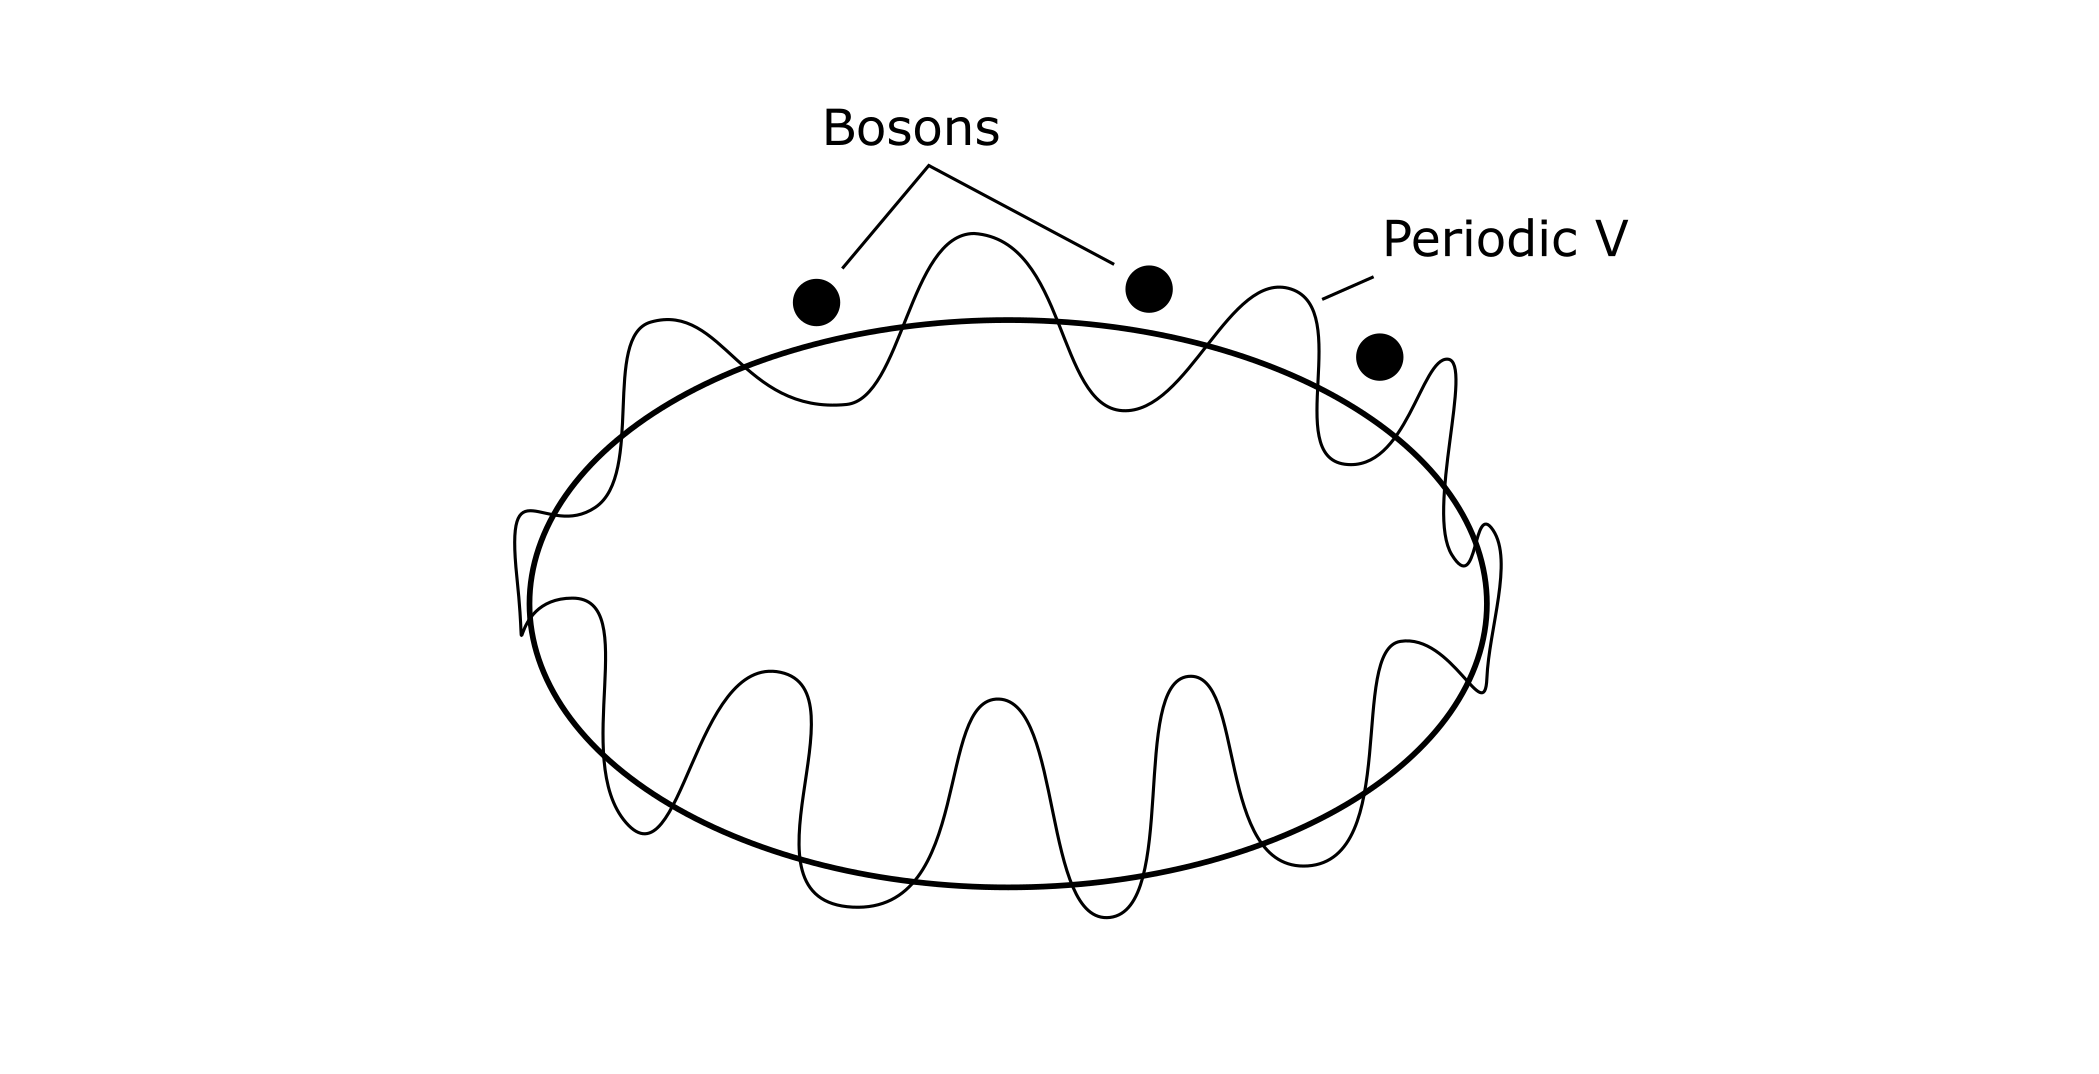
\includegraphics[width=\linewidth]{Figures/bose_hubbard.png}
    \caption*{}
    \label{fig:bhub}
\end{figure}

In this system we set the number of minima ('valleys') in the potential to be $N$. We then make lots of approximations to the general form of the Hamiltonian:
\[H = \int \dd^3 x \Psi^\dagger(x)(T-V_0)\Psi(x) + \iint \dd^3 x \dd^3 y \Psi^\dagger(x)\Psi^\dagger(y)V\Psi(x)\Psi(y)\]
The first term is the kinetic energy of the particle - particles may tunnel between minima. The second term in the Hamiltonian, $J\sum_{j=0}^{N-1}a_j^\dagger a_j(a_j^\dagger a_j - \II)$, is the repulsion term - it represents Bosons being pushed away from the potential. The third term, $ \mu\sum_{j=0}^{N-1}a_j^\dagger a_j$. is the chemical potential term which tells you that particles will want to enter the system from the outside. If you want eternal fame and glory you could try and exactly solve this model, but you might not learn a lot! It turns out that the variational method and perturbation theory have taught us an extraordinary amount about this model. So let's try this with the variational method. I can say safely that there are thousands of papers on the solutions of this model.

Okay, so let's start with the variational class. $V =\{\ket{\alpha}:\alpha=(\alpha_1,...,\alpha_N);\alpha_j \in \CC;j\leq N\}$. Then we set:
\[E^* = \inf_{\ket{\alpha} \in V}\expval{H_{\textrm{BHM}}}{\alpha}\]
We can exploit the fact that under $j\mapsto j+1$ we have $H \mapsto H$ due to the rotational symmetry here. It's reasonable to expect that the useful kets in $V$ will respect that symmetry. So we will use $V_{TI}\subset V$ where we have $V_{TI} = \{\ket{\alpha}:\alpha=(\alpha_0,\alpha_0,...\alpha_0);\alpha_0\in\CC\}$. These are the kets which are rotationally invariant in this system. You have to be very careful about adding these symmetries to the Variational method - sometimes there is symmetry breaking! But we claim that this variational class is a good start to looking at this model. Okay, let's compute the expectation value now. We will break it into steps.
\begin{align}
\expval{-t\sum_{j=0}^{N-1}a_{j+1}^\dagger a_j}{\alpha} &= -t\sum_{j=0}^{N-1}|\alpha|^2\\
&= -2Nt|\alpha|^2
\end{align}
\begin{align}
\expval{a_j^\dagger a_j a_j^\dagger a_j}{\alpha} &= |\alpha|^2 \expval{a_j a^\dagger_j}{\alpha}\\
&= |\alpha|^2 \expval{\II + a_j^\dagger a_j}{\alpha} \\
&= |\alpha|^2 (1+|\alpha|^2)
\end{align}
All together now, we get the following value (the chemical potential term is the same difficulty to calculate as the first term).
\begin{equation}
\expval{H}{\alpha} = -2Nt|\alpha|^2 + NJ(|\alpha|^2(1+|\alpha|^2)) - JN|\alpha|^2 + \mu N |\alpha|^2
\end{equation}
Now we take the infimum over all $\alpha$. This is easier if we choose polar coordinates, $\alpha = re^{i\theta}$.
\begin{align}
E^* &= \inf \expval{H}{\alpha}\\
&= \inf_{r\in \RR^+} \left(-2Ntr^2 +NJ(r^2+r^4) - JNr^2 +\mu Nr^2 \right)\\
&= \inf_{x\in \RR^+} \left(-2Ntx +NJ(x+x^2) - JNx +\mu Nx \right)\\
&= \inf_{x\in \RR^+} \left((-2Nt+\mu N)x + NJx^2\right)\\
&= N \inf_{x\in \RR^+} x(Jx - 2t+\mu)
\end{align}
\begin{align}
\pdv{x}( x(Jx+2t-\mu))&=-(-Jx+2t-\mu)+Jx\\
&=0\\
\implies x &= \frac{2t-\mu}{2J}
\end{align}
This is very easy! It's just the minimization of a quadratic. This isn't going to be as easy as a quadratic - but in general you can just use an optimization program to reduce this problem. What this tells us is that as long as $\mu>2t$ (that is: the chemical potential is large enough to place bosons into the system) we have a solution for the approximate ground state, which we can find the remaining states from through applying orthogonality. It is:
\[\alpha = \left(\frac{2t-\mu}{2J}\right)^{1/2}e^{i\theta}\]
\subsubsection{Coherent States for Quantum Fields}
\begin{defn}[Displacement Operator]
We define the Displacement Operator as follows. Let $\phi : \RR^3 \to \CC$ (this is essentially the Fourier series version of $\ket{\alpha}$ with $\alpha_i$ as coefficients).
\begin{equation}D(\hat\Psi,\phi) = \exp\left(\int \dd^3 x \phi(x)\hat\Psi^\dagger(x) - \overline \phi(x)\hat\Psi(x)\right)\end{equation}
\end{defn}
\begin{defn}[Field Coherent State]
A field coherent state is then
\begin{equation}\ket{\phi} = D(\hat\Psi,\phi)\ket{\Omega}\end{equation}
\end{defn}

What we hope is that somehow these are eigenstates of the quantum field operators:
\begin{equation}
\hat\Psi(x)\ket{\phi} = \phi(x) \ket{\phi}
\end{equation}
To see this, begin with the commutator $[\hat\Psi(x),D(\hat\Psi,\phi)]$. Then apply the fact that $\hat\Psi(x)\ket{\Omega}=0$. We look at $\hat\Psi(s,x) = D^{\dagger s}\hat \Psi(x)D^s$ (where $s \in [0,1]$). We then set up a differential equation:
\begin{align*}
\pdv{s}\hat\Psi(s,x) &= \pdv{s}\left(\exp{-s\int \dd^3 x (\phi\hat\Psi^\dagger-\overline\phi\hat\Psi)} \hat\Psi(x) \exp{s\int \dd^3 x (\phi\hat\Psi^\dagger-\overline\phi\hat\Psi)}\right)\\
&= -\int \dd^3 x (\phi\hat\Psi^\dagger-\overline\phi\hat\Psi) \left(\exp{-s\int \dd^3 x (\phi\hat\Psi^\dagger-\overline\phi\hat\Psi)} \hat\Psi(x) \exp{s\int \dd^3 x (\phi\hat\Psi^\dagger-\overline\phi\hat\Psi)}\right)\\
&+\left(\exp{-s\int \dd^3 x (\phi\hat\Psi^\dagger-\overline\phi\hat\Psi)}\hat\Psi(x)  \int \dd^3 x (\phi\hat\Psi^\dagger-\overline\phi\hat\Psi) \exp{s\int \dd^3 x (\phi\hat\Psi^\dagger-\overline\phi\hat\Psi)}\right)\\
&= -\int \dd^3 x (\phi\hat\Psi^\dagger-\overline\phi\hat\Psi) D^{\dagger s} \hat\Psi(x)D^s+ D^{\dagger s}\hat\Psi(x)\int \dd^3 x (\phi\hat\Psi^\dagger-\overline\phi\hat\Psi)D^s
\end{align*}
Note that $[\exp(A),A] = 0$ from the following identity:
\[[A,\exp{B}]= \int_0^1 \dd s \exp{(1-s)B}[A,B]\exp{sB}\]
Then we have the following.
\begin{align*}
\pdv{s}\hat\Psi(s,x) &= -\int \dd^3 x (\phi\hat\Psi^\dagger-\overline\phi\hat\Psi) D^{\dagger s} \hat\Psi(x)D^s+ D^{\dagger s}\hat\Psi(x)\int \dd^3 x (\phi\hat\Psi^\dagger-\overline\phi\hat\Psi)D^s\\
&= D^{\dagger s} [\hat\Psi(x),\int \dd^3 y \phi(y)\hat\Psi^\dagger(y)-\overline\phi(y)\hat\Psi(y)]D^s\\
[\hat\Psi(x),\int \dd^3 y \phi(y)\hat\Psi^\dagger(y)-\overline\phi(y)\hat\Psi(y)] &= \int \dd^3 y \hat\Psi(x)\phi(y)\hat\Psi^\dagger(y)-\hat\Psi(x)\overline\phi(y)\hat\Psi(y)\\
&= \int\dd^3 y \phi(y)([\hat\Psi(x),\hat\Psi^\dagger(y)]-[\hat\Psi(x),\hat\Psi(y)]\\
&= \int \dd^3 y \phi(y)(0-\delta(x-y))\\
&= -\phi(x)
\end{align*}
Putting this together tells us:
\begin{equation}
\Psi(1,x)=D^\dagger \hat\Psi(x) D = -\phi(x)\hat\Psi(x)
\end{equation}
\[[\hat\Psi,D(\hat\Psi,\phi)] = (\phi-1)D(\hat\Psi,\phi)\hat\Psi\]
\[\implies [\hat\Psi,D(\hat\Psi,\phi)]\ket{\Omega} = (\phi-1)D(\hat\Psi,\phi)\hat\Psi\ket{\Omega}\]
\begin{align}
\implies \hat\Psi(x) D(\hat\Psi(x),\phi(x))\ket{\Omega} - D(\hat\Psi(x),\phi(x))\hat\Psi(x)\ket{\Omega} &= (\phi(x)-1)\ket{\phi}\\
\hat\Psi(x)\ket{\phi}-\ket{\phi}=(\phi(x)-1)\ket{\phi}\\
\hat\Psi(x)\ket{\phi}=\phi(x)\ket{\phi}
\end{align}
Now we begin the variational calculation using these states. Let our variational class to be all field coherent states which are twice differentiable.
\begin{align}
E^* &= \inf_{\ket{\phi}\in V} \expval{\dd^3 x \hat\Psi^\dagger(x)(T(x)-V_0(x))\hat\Psi(x) + \frac{1}{2}\iint\dd^3 x \dd^3 y \hat\Psi^\dagger(x)\hat\Psi^\dagger(y)V(x,y)\hat\Psi(x)\hat\Psi(y)}{\phi}\\
&= \inf_{\phi}\int \dd^3 x\overline\phi(x) (T(x)-V_0(x))\phi(x)+\frac{1}{2} \iint \dd^3 x \dd^3 y \overline\phi(x)\overline\phi(y)V(x,y)\phi(x)\phi(y)
\end{align}
This is a functional of some $\phi$! This means that this is now just a problem in the calculus of variations. We needed $\phi$ to be twice differentiable because $T = \frac{-\hbar^2}{2m}\nabla^2$. So now we let our Action be the following.
\[S[\phi,\partial_x \phi, \partial_x^2 \phi] =\int \dd^3 x\overline\phi(x) (T(x)-V_0(x))\phi(x)+\frac{1}{2} \iint \dd^3 x \dd^3 y \overline\phi(x)\overline\phi(y)V(x,y)\phi(x)\phi(y)\]
Which gives us the Euler-Lagrange equations:
\begin{equation}
\pdv{S}{\phi}-\pdv{x}\pdv{S}{\partial_x\phi} = 0
\end{equation}
As a simple example, we can take $V(x,y) = \kappa \delta^{(3)}(x-y)$. This gives a very special form for the equations of motion: the Time-Independent Gross-Pitaevskii Equation.
\begin{equation}
L[\phi]=0\implies \left(\frac{-\hbar^2}{2m}\nabla^2 + V_0(x)\right)\phi(x) + \kappa|\phi(x)|^2 \phi(x)=0
\end{equation}

Next we will consider another system, the degenerate electron gas. This is appropriate for a plasma or a metal.

\subsection{Degenerate Electron Gas}
We will begin with electrons in a box with periodic boundary conditions. Eventually we will take the side length of the box to infinity, but we must be careful to not get divergences.

In the single particle basis we have the following wave functions:
\[\phi_{k,\alpha}(x)=\frac{1}{V}\exp\left(ik\cdot x\right)\eta_\alpha\]
\[\eta_+ = (1,0), \eta_-=(0,1)\]
We know that for these plane waves the $k_i$ components must be proportional to integers: $k_i =\frac{2\pi}{L}n$. We have chosen the label $\eta$ for the internal degree of freedom for the particle (here being spin). Now we will find the second quantized Hamiltonian for this system. This is a very elegant example - we will simply add the coulomb potential as a perturbation and immediately get numbers comparable with experiment. Our Hamiltonian will look something like the following.
\begin{equation}
    H = H_{electrons}+H_{background}+H_{interaction}
\end{equation}
To do this calculation correctly, we need to pick a background. The background is chosen to make the system electrically neutral. We are going to be thinking about a lot of electrons, in fact, we will think about the number of electrons in the system going to infinity. To model real world materials we must always take into account that the electrons are moving in a background potential such as a lattice of atoms. This background makes the system stable - imagine a $1$-Farad capacitor, charged completely. If you short this capacitor you will see a blinding flash! A huge kablam. This is not desirable, because this is quite an unstable effect. Let's choose the background to be a classical field for a decent approximation, so that we can focus on $H_{el}$. This is going to be a kinetic energy term plus a potential energy term as usual. We start with the kinetic energy:
\[T = \sum_{\alpha, \beta}\int \dd^3 x \dd^3 y \hat\Psi^\dagger_\alpha(x)\left(\frac{-\hbar^2\nabla^2}{2m}\right)\hat\Psi_\beta(y)\]
Here $\alpha$ and $\beta$ label spin.
\[V = \sum_{\alpha_1,...,\alpha_4}\int \dd^3 x\dd^3 y \hat\Psi_{\alpha_1}^\dagger(x)\hat\Psi_{\alpha_2}^\dagger(y)\hat\Psi_{\alpha_3}(y)\hat\Psi_{\alpha_4}(x)V_{\alpha}(x,y)\]
This $V$ is given by some kind of coulomb interaction. We won't deal with relativistic effects, so we assume the interaction happens instantaneously. Classically, this is the potential (we will later take $\mu \to 0$):
\[V_c(x,y)=\frac{\exp(-\mu|x-y|)}{|x-y|}\delta_{\alpha_1\alpha_4}\delta_{\alpha_2\alpha_3}\]
The right approach is to first take the system to be finite, then take the size of the box to be large, then set the constant $\mu$ to zero. We will take the background to be pretty much constant - the atoms are so heavy relative to the electrons that they don't move around very much, so by an Adiabatic approximation we will just assume that they don't change. There are occasionally situations where the response of the atoms are crucial - such as in superconductivity. The reason superconductivity occurs is that electrons can interact with the low energy phonons in a substance - hence the motion of atoms is significant. This background interaction Hamiltonian is given by the following.
\begin{equation}
    H_{interaction} = -e^2 \int \dd^3 x \dd^3 y  n_b(x) \frac{\exp(-\mu|x-y|)}{|x-y|}n_e(y)
\end{equation}
As an exercise, prove that this Hamiltonian reduces to a constant:
\[H_{interaction} = e^2\frac{N^2}{V}\frac{4\pi}{\mu^2}\]
Where $N$ is the number of electrons. Note that we assume this is definite for this case. Similarly, the background itself is given by the following:
\begin{equation}
H_b = \frac{1}{2}e^2\int\dd^3 x \dd^3 y n_b(x) n_b(y)\frac{\exp(-\mu|x-y|)}{|x-y|}
\end{equation}
Note that we choose $n_b(x)$ to be translation invariant so it is just a number. You should also prove that the second integral reduces to the following.
\[\frac{1}{2}e^2 \frac{N^2}{V}\frac{4\pi}{\mu^2}\]
Let's work out the matrix elements of the last term now, as they will allow us to work out the full second quantized Hamiltonian. The kinetic energy matrix elements are pretty simple:
\[\mel{\phi}{T}{\phi'}=\mel{\phi}{-\frac{\hbar^2\nabla^2}{2m}}{\phi'} = \frac{1}{2mV}\int \dd^3 x e^{-ikx}\eta_\alpha^* T \eta_\beta e^{i\ell x} = |\ell|^2\frac{-1}{2mV}\hbar^2\int \exp(i(\ell x - kx))\delta_{\alpha \beta} = \frac{\hbar^2}{2m}|k|^2\delta_{\alpha \beta}\delta_{k \ell}\]
\begin{equation}
T =\sum_{k,\alpha} \frac{\hbar^2 |k|^2}{2m}a^\dagger_{k,\alpha}a_{k,\alpha}
\end{equation}
Some notation we will see often is $|\vec{k}|^2 = k^2$. We will next compute the potential energy elements:
\[\bra{\phi_{k_1,\alpha}}\bra{\phi_{k_2,\beta}}V\ket{\phi_{k_3,\gamma}}\ket{\phi_{k_4,\delta}}= \frac{e^2}{V^2}\int\dd^3 x\dd^3 y e^{-i(k_1-k_2)x}(\eta_\alpha^\dagger \otimes \eta_\beta^\dagger)\frac{e^{-\mu|x-y|}}{|x-y|}(\eta_\gamma\otimes \eta_\delta)e^{-i(k_3-k_4)y}\]
To compute this integral, first we make a change of variables $z = x-y$:
\[\bra{\phi_{k_1,\alpha}}\bra{\phi_{k_2,\beta}}V\ket{\phi_{k_3,\gamma}}\ket{\phi_{k_4,\delta}}= \frac{e^2}{V^2}\delta_{\alpha \gamma}\delta_{\beta \delta'}\int \dd^3 y \dd^3 z e^{-i(k_1+k_2-k_3-k_4)y}e^{i(k_3-k_1)z}\frac{e^{-\mu|z|}}{|z|}\]

\nocite{*}
\printbibliography
\end{document}







